\def\degre{^{\circ}}

\section*{Introduction}

     Global three-dimensional chemistry-transport models (hereafter
     referred to as CTMs) play an important role in monitoring and
     predicting the composition of the atmosphere
     \citep[e.g.,][]{Chipperfield2006,Teyssedre2007,Huijnen2010}. Those
     models include large-scale transport, emissions and chemical
     transformations of trace species, and sub-scale grid processes
     like convection and deposition. In CTMs, advection by large-scale
     winds is a~key process that must be handled by numerical
     algorithms. For these algorithms, mass conservation for
     the considered species, monotonicity and numerical accuracy are
     especially important for long simulations where accumulation of
     errors and bias must be avoided.

     In this paper, we present a~conservative advection model on the
     sphere which is intended to form the basic framework for
     a~future CTM. The adopted scheme is based on a~flux-form
     (Eulerian) tracer advection algorithm on a~reduced
     latitude--longitude grid. A~finite-volume approach was chosen as
     it provides an easy way to ensure mass preservation. Furthermore,
     parallelizing the model is then reduced to a classical domain decomposition
     problem.

     The specificity of our model, named Pangolin\footnote{PArallel
       implementatioN of a~larGe scale multi-dimensiOnaL
       chemIstry-traNsport scheme}, lies in the grid definition, where
     the number of cells on a~latitude circle is progressively
     decreased towards the pole in order to obtain a~grid which approximately
     preserves the cell areas at mid- and
     high latitudes. This avoids the so-called ``pole problem''
     arising from the convergence of the meridians, which severely
     limits the size of the time steps for Eulerian models. Several
     approaches have been adopted in previous studies to cope with
     this issue. Finite-volume schemes on latitude--longitude grids
     often aggregate latitudinal fluxes near the poles
     (e.g.,~\cite{Hourdin1999}) or successively double the grid size
     at high latitudes (e.g., ~\cite{Belikov2011}).


     Alternatively, quasi-uniform spherical grids have been developed,
     such as a cubed-sphere\footnote{Each face uses Cartesian
       coordinates and is projected gnomonically or conformally on the
       sphere.}, composite mesh -- Yin-Yang -- or icosahedral
     grids\footnote{An icosahedra is subdivided until the desired
       resolution and projected on the sphere.}. A~review of the
     different grids can be found in~\citet{Staniforth2012}
     and~\citet{Williamson2007}. However, those approaches lose the
     latitudinal regularity arising from the rotation of the Earth.
     Furthermore, they require specific treatments at the
     singularities of the adopted polygons, which may also induce
     resolution clustering near these points. On the plus side, they
     allow for the implementation of more accurate algorithms than the
     ones on reduced latitude--longitude grids. This last point is
     especially important for weather and climate models that solve
     the nonlinear momentum equation, but is less stringent for the
     two-dimensional (2-D) linear transport of trace species on the
     sphere.


     To construct the reduced grid, one difficulty is to define
     a~structure which avoids treating the poles as special cases, as
     that can impact the precision and properties of the advection
     algorithm. Thus we have chosen to adopt a~semi-structured
     approach. The grid is not regular as the number of cells varies
     with the latitude, but the coordinates of cell interfaces can be
     computed algebraically.  We thus avoid storing a~list of
     neighbors as an irregular unstructured grid would normally
     require, hence decreasing memory costs. This was done to
     anticipate future parallel architectures, which may have less
     memory capacity per core than current systems.

     Our goal is to use an adequate algorithm exploiting the grid
     features to achieve efficiency and scalability on massively
     parallel architectures. Fine control over parallelization was
     obtained using the Message Passing Interface (MPI) library.  In
     that context, the advection scheme must be chosen as to balance
     its accuracy vs. the volume of the required parallel communications.
     Furthermore, grid properties were carefully studied to improve
     the parallel version.  In particular, a~custom domain decomposition
     consistent with our grid was designed.

     The present paper is organized as follows. Section~\ref{sec2:scheme}
     lists the basic equations and numerical methods used to solve
     the advection of the chemical species. In Sect.~\ref{sec2:tests},
     results from standard test cases for advection of tracer on the
     sphere are reported. Those cases were chosen from the test case
     suite proposed by~\citet{Lauritzen2012}. Section~\ref{sec2:parallel}
     gives details on the model implementation on parallel
     architectures and the results of parallel scalability experiments. In
     Sect.~\ref{sec2:ccl}, we summarize the results obtained and discuss the
     possible extension of our method.


\section{Numerical scheme}
\label{sec2:scheme}
   \subsection{Finite-volume formulation}

   Our model is based on a~finite-volume method to integrate the
   tracer advection equation. This is performed on a~bi-dimensional
   discrete grid on the sphere, which is described in more detail in
   Sect.~\ref{subsec:grid}. In each grid cell, the tracer
   concentration changes according to the divergence of the fluxes at
   the cell boundaries. This comes from the flux form of the
   continuity and tracer conservation equations:
   \begin{align}
     &\frac{\partial \rho}{\partial t} + \nabla \cdot (\rho \vec{V}) = 0 ,
     \label{eqn:air2}
     \\
     &\frac{\partial \rho q}{\partial t} + \nabla \cdot ( \rho q \vec{V})  = 0,
     \label{eqn:tracer2}
   \end{align}
   where $\rho$ is the air density, $q$ the tracer mixing ratio and
   $\vec{V}$ the winds vector field. Equations~(\ref{eqn:air2}) and
   (\ref{eqn:tracer2}) are first integrated over a~cell area
   $\mathcal{A}$. With $\partial\mathcal{A}$ noted as the cell boundary and
   $\vec{n}$ as the local normal pointing outward, the divergence theorem yields
   \begin{align}
     &\frac{\partial m}{\partial t}=\frac{\partial}{\partial t} {\int_{\mathcal{A}}
   \rho}
   = \int_{\partial \mathcal{A}} (\rho \vec{V}\cdot\vec{n} \;\mathrm{d}S),
   \label{eqn:air3}
   \\
   &\frac{\partial m_r}{\partial t}=\frac{\partial}{\partial t} {\int_{\mathcal{A}}
 \rho q} = \int_{\partial \mathcal{A}} (\rho q \vec{V}\cdot \vec{n} \;\mathrm{d}S),
 \label{eqn:tracer3}
     \end{align}
     where ${m}$ is the total air mass in a~cell and ${m_r}$ is the
     total tracer mass in a~cell. The right-hand side of
     Eqs.~(\ref{eqn:air3}) and (\ref{eqn:tracer3}) can be seen as the
     integral of all the fluxes across the cell boundaries. This
     formulation gives a~conservative scheme when the same fluxes are
     used for upstream and downstream adjacent cells.

     The above equations are then integrated in time during
     a~time step:
     \begin{align}
       &m^{n+1} = m^{n} - \int_{t_n}^{t_{n+1}}
       \Big( \int_{\partial \mathcal{A}} \rho \vec{V}\cdot\vec{n}\;\mathrm{d}S \Big) \mathrm{d}t,
       \label{eqn:mintegral}
       \\
       &m_r^{n+1} = m_r^{n} - \int_{t_n}^{t_{n+1}}
       \Big( \int_{\partial \mathcal{A}} \rho q \vec{V}\cdot\vec{n}\;\mathrm{d}S \Big) \mathrm{d}t.
       \label{eqn:qintegral}
   \end{align}
   Equation~(\ref{eqn:mintegral}) can be omitted for non-divergent flows since
   the divergence of the mass fluxes is null and the mass inside the cells is
   constant: $[m]^{n+1} = [m]^{n}$. In this paper, we only consider
   non-divergent flows. As such, winds are corrected to be divergence-free in a
   preprocessing step, as explained in Sect.~\ref{subsec:adapting}.  Handling
   divergent flows would require minor adjustments to the scheme (removing the
   correction of winds and adding Eq.~\eqref{eqn:mintegral} to the scheme), but
   this configuration was not considered as a typical use case of CTMs, where
   large-scale 3-D winds can be considered divergence-free.

   There are many options to evaluate the tracer mass fluxes at the
   cell boundary. These fluxes are approximated as the air mass fluxes
   multiplied by the mean tracer ratio $\widehat{q}$ crossing the
   interface. The simplest approach to evaluate $\widehat{q}$ was
   introduced by Godunov~\citep{Godunov1961}, who considered $\widehat{q}$
   as constant within each upstream cell. The resulting scheme is
   conservative and monotonicity preserving but very diffusive. Improvements to the
   Godunov scheme were introduced by van Leer
   in~\citet{Leer1977}, where $q$ is now approximated by
   a~non-constant polynomial function. Depending on the polynomial
   degree used, i.e., the order moments of the distribution of $q$
   inside the cell, van Leer obtained several schemes (up to six) that
   varied in complexity. A~review of the different possible options
   can be found in~\citet{Rood1987} and \citet{Hourdin1999}.  In
   general, accuracy is found to increase when higher-order moments
   are used, but the price to pay lies in larger computational and
   memory costs. Using higher moments requires a larger number of
   grid points to compute the derivatives, which increases communication volumes
   when domain decomposition techniques are used for parallel clusters (see
   Sect.~\ref{sec2:parallel}).


%f1
\begin{figure}[t]
  \begin{centering}
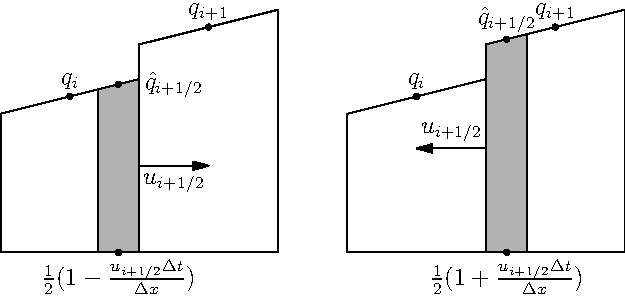
\includegraphics[width=8.5cm]{gmd-2014-119-f01.pdf}
\caption{Van Leer scheme for positive (left) and negative (right) winds. The distribution of the
tracer is shown as a linear distribution (broken line). The grey area is the
quantity of tracer passing through the interface during a~time step.}
\label{fig2:van_leer}%
  \end{centering}
\end{figure}%




   For our model, we have adopted a~first-order reconstruction, the
   van Leer scheme (noted as van Leer I in the original paper). The
   distribution of $q$ in the cells is approximated by a~linear
   function in latitudinal and meridional directions. The slope of the
   linear function is computed as a~finite difference using the values
   of $q$ within the nearest cells. In that configuration, the scheme
   is second-order accurate in space. To extend the algorithm to multiple
   dimensions, a~time-splitting scheme is
   used. Equations~(\ref{eqn:mintegral}) and (\ref{eqn:qintegral}) are
   first integrated in the zonal direction:
   \begin{align}
     &   \widetilde{m}_i^{n+1} = m_i^{n} + U_{i-1/2} - U_{i+1/2},\nonumber \\
     &   (\widetilde{m_r})_i^{n+1} = (m_r)_i^{n} + F_{i-1/2} - F_{i+1/2},
     \label{eqn:flux}
   \end{align}
   where $U$ and $F$ are the air and tracer fluxes, respectively, across
   the borders orthogonal to the chosen direction during
   a~time step. With these notation, tracer fluxes are approximated
   as $F_{i+1/2} \approx \widehat{q}_{i+1/2} u_{i+1/2}$.
   Figure~\ref{fig2:van_leer} illustrates the reconstruction of
   $\widehat{q}_{i+1/2}$.  The linear distribution represents the tracer
   distribution in the 1-D case for cells $i$ and $i+1$. Finding
   $\widehat{q}_{i+1/2}$ depends on the wind direction: for outward winds
   ($u_{i+1/2} > 0$), the grey area in the left diagram will move from
   cell $i$ to cell $i+1$. Then the mean tracer ratio corresponding to
   this flux is computed from the distribution in cell $i$.  The same
   can be applied for inward fluxes, resulting in
   \begin{align*}
     \widehat{q}_{i+1/2} =
     \begin{cases}
       q_i + \left(1 -  \frac{u_{i+1/2} \Delta t}{\Delta x}\right)(\delta q)_i
       \quad &\text{if} \quad u_{i+1/2} > 0,\\
       q_{i+1} - \left(1 + \frac{u_{i+1/2} \Delta t}{\Delta x}\right) (\delta q)_{i+1}
       \quad &\text{otherwise},
     \end{cases}
   \end{align*}
   where $\delta q$ is the slope of the linear reconstruction and
   $u_{i+1/2}$ the wind at the interface. $\Delta t$ and $\Delta x$
   are the time step and cell spacing, respectively.

   This first advection step gives us the intermediate mass value
   $\widetilde{m}$ and tracer value
   $q'=\widetilde{m}/\widetilde{m_r}$. These new values are then used
   to integrate Eq.~(\ref{eqn:qintegral}) in the meridional direction.
   As the grid is unstructured, mass and tracer fluxes in the
   north--south direction have to be evaluated for all the neighbors
   of each cell. This is detailed in Sect.~\ref{subsec:adapting}.


%f2
\begin{figure*}[t]
  \begin{centering}
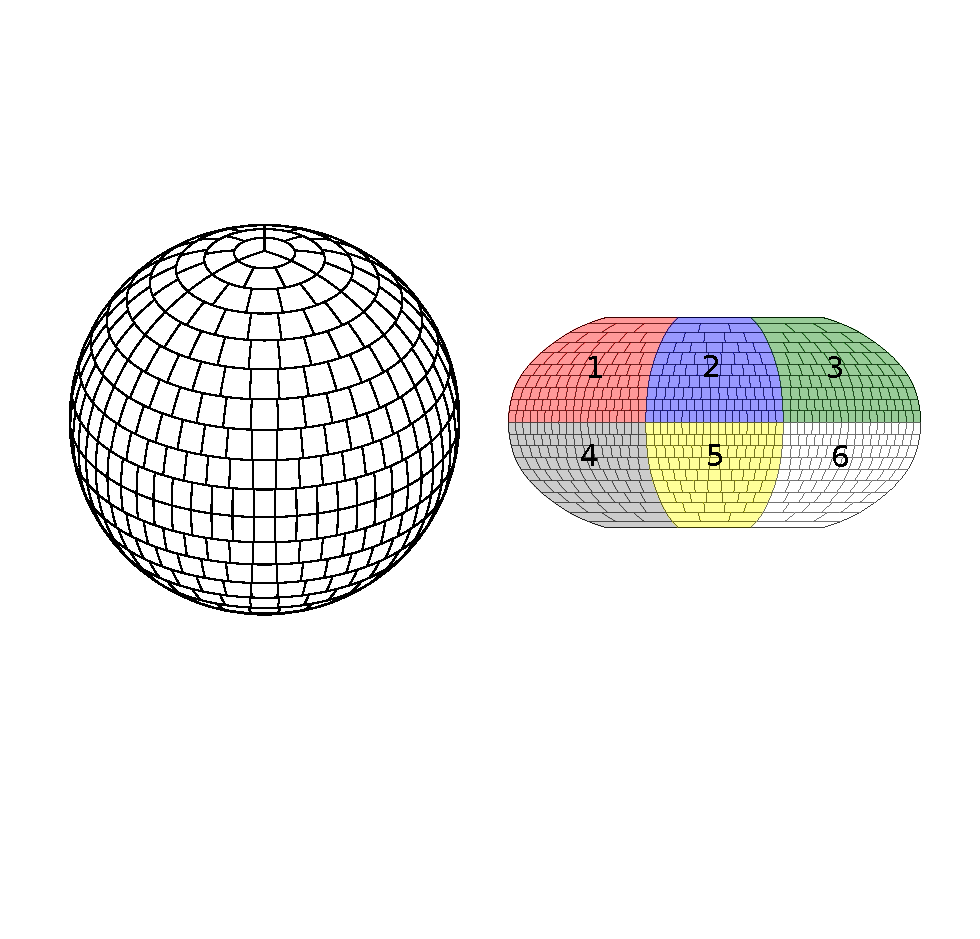
\includegraphics[width=12cm]{gmd-2014-119-f02.pdf}
\caption{Grid used in Pangolin with 20 latitudes: orthographic projection
    (left) and Robinson projection, with the six identical zones highlighted
  (right).}
\label{fig2:pango_grid}%
  \end{centering}
\end{figure*}


   It should be noted that other time-splitting schemes are available. Another
   approach is to use a~zonal--meridional advection during a~time step and
   meridional--zonal for the next. It is also possible to compute both
   zonal--meridional and meridional--zonal advection and then use their mean as
   the final value. For the complete description of each method, see
   \citet{Machenhauer2009}. Either way, the final bidimensional algorithm is
   second-order accurate. In Pangolin, all three time-splitting schemes
   have been tested using the numerical order of convergence test  (see
   Sect.~\ref{subsec:conv}). It was found the choice of the time-splitting
   algorithm has little impact on accuracy.

   To ensure monotonicity of the solution and to prevent numerical
   oscillations, van Leer introduced a~slope limiter. The idea is to
   limit the slope value within a~given cell such as the tracer value
   in that cell does not exceed the mean value of the adjacent
   cells. This is more restrictive than limiting the fluxes to ensure
   that the tracer values remain between the maximum--minimum values of
   the adjacent cells but is easier to implement. The slope is given
   by
   \begin{equation}
     (\delta q)_i =
     \min\Big(\frac{1}{2} |q_{i+1}-q_{i-1}|, 2|q_{i+1}-q_i|, 2|q_i-q_{i-1}|\Big)
     \quad \times \text{sign}(q_{i+1} - q_i)
     \label{eqn:slope2}
   \end{equation}
    if $q_i$ lies in between $q_{i-1}$ and $q_{i+1}$, and $(\delta
    q)_i =0$ otherwise.  As discussed by~\citet{Hourdin1999}, the
    slope limiter efficiently damps the numerical oscillations but
    introduces more diffusion of the numerical solutions. For the test
    cases reported in this study, the slope limiter appears to have
    little impact on the accuracy of the numerical solutions.



\subsection{Grid}
    \label{subsec:grid}


    The grid used in Pangolin is completely defined by the number of
    cells at the North Pole and the number of latitudes
    $n_{\text{lat}}$ on a hemisphere. The Southern Hemisphere is
    simply constructed in the same way as the Northern Hemisphere. To
    find the number of cells at the North pole, we can write the equality
    between cell areas at the pole and at the Equator. If we consider
    squared cells at the Equator, like the ones on a~regular
    latitude--longitude grid, and small latitudinal spacing, the number
    of cells is approximately $\pi$. Thus we set the number of cells
    at the poles to 3.



    At a~given latitude, all cells have the same area. We can then
    compute the number of cells for all latitudes. For
    maximum flexibility, latitudinal and longitudinal spacings are no longer assumed identical. Let us consider the area of cell $(i,j)$,
    noted $\mathcal{A}_{i}$ as it does not depends on $j$. Let us note
    $\phi_i$ as the colatitude and $\lambda_{ij}$ as the position of the
    south and east cell borders. As we assume that the cell spacings are
    constant, we can write $\phi_i =i\Delta\phi_i$ and
    $\lambda_{ij}=j\Delta\lambda_i$.  The area is defined on
    $\Omega_{ij} = [\lambda_j, \lambda_{j+1}]\times
    [\phi_{i-1},\phi_i]$, so in spherical coordinates we have
\begin{align}
\mathcal{A}_{i} &= \iint_{\Omega_{ij}}  r^2 \sin\phi \mathrm{d}\lambda \mathrm{d}\phi \nonumber\\
  &= r^2 \Delta\lambda_i \big (\cos(\phi_{i-1}) - \cos(\phi_{i-1}+\Delta\phi_i)\big).
\label{eqn:cell_area}
   \end{align}

   Areas are preserved so $\mathcal{A}_i=\mathcal{A}_1$:
\begin{align*} \Delta\lambda_i  = \Delta\lambda_1 \frac {1-\cos(\Delta\phi_1)}
{2\sin\left( \frac{\Delta\phi_i}{2} \right) \sin\left(\left(i-\frac{1}{2}\right)\Delta\phi_i\right)}.
   \end{align*}

   Noting $n_i$ the number of cells at colatitude $i$, we get
\begin{align*} \frac{n_i}{n_1} = \left\lfloor \frac{\Delta\lambda_1}{\Delta\lambda_i} \right\rfloor=
\left\lfloor \frac {2\sin\left( \frac{\Delta\phi_i}{2} \right) \sin\left(\left(i-\frac{1}{2}\right)\Delta\phi_i\right)}%
{1-\cos(\Delta\phi_1)}\right\rfloor.
   \end{align*}

   Now let us assume $\forall i$, $\Delta\phi_i$ and
   $(i-\frac{1}{2})\Delta\phi_i$ are small enough:
\begin{align*} \frac{n_i}{n_1} \approx
\left\lfloor \frac{2  \frac{\Delta\phi_i}{2}  \left(i-\frac{1}{2}\right) \Delta\phi_i}%
{ \frac{\Delta\phi_1^2}{2}} \right\rfloor
= 2i-1.
   \end{align*}

   Finally, we can define the number of cells for the whole grid, with
   $2n_{\text{lat}}$ latitudes, as
\begin{align}
&n_i =
    \begin{cases}
      3(2i-1) & \quad \text{if} \; 1 \le i \le n_{\text{lat}}, \\
      n_{2n_\mathrm{lat}-i+1} & \quad \text{otherwise.}
    \end{cases}
    \label{eqn:nb_cells2}
   \end{align}

   It follows that the total number of cells on the grid is
   $6n_{\text{lat}}^2$. As an illustration, the grid is shown in
   Fig.~\ref{fig2:pango_grid}.




   The previous formula is a~sound approximation for area preservation near the
   poles and when latitudinal spacing is constant.  In practice, we consider the
   approximation as reasonable up to 75\degree: the relative error is
   then less than 1\,\%. At lower latitudes, the error
   increases, with a~maximum of 56\,\% at the Equator. So the
   grid used in Pangolin gives higher resolutions at the Equator than
   at the poles.  One way around this issue is to truncate the number
   of cells at a~given threshold.  As a~comparison,
   Fig.~\ref{fig2:nb_cells} shows the number of cells for Pangolin with
   the ``exact'' and truncated version. By ``exact'', we mean the number
   of cells comes from the area-preservation formulae without any
   approximations for $\Delta\phi_i$.  Furthermore, to truly preserve
   the cell areas, we should use a~variable latitudinal spacing.
   However, the distortion due to a~constant latitudinal spacing was
   found to be acceptable and much less pronounced compared with
   a~regular latitude--longitude grid.

%f3
\begin{figure}
  \begin{minipage}[t]{0.48\linewidth}
%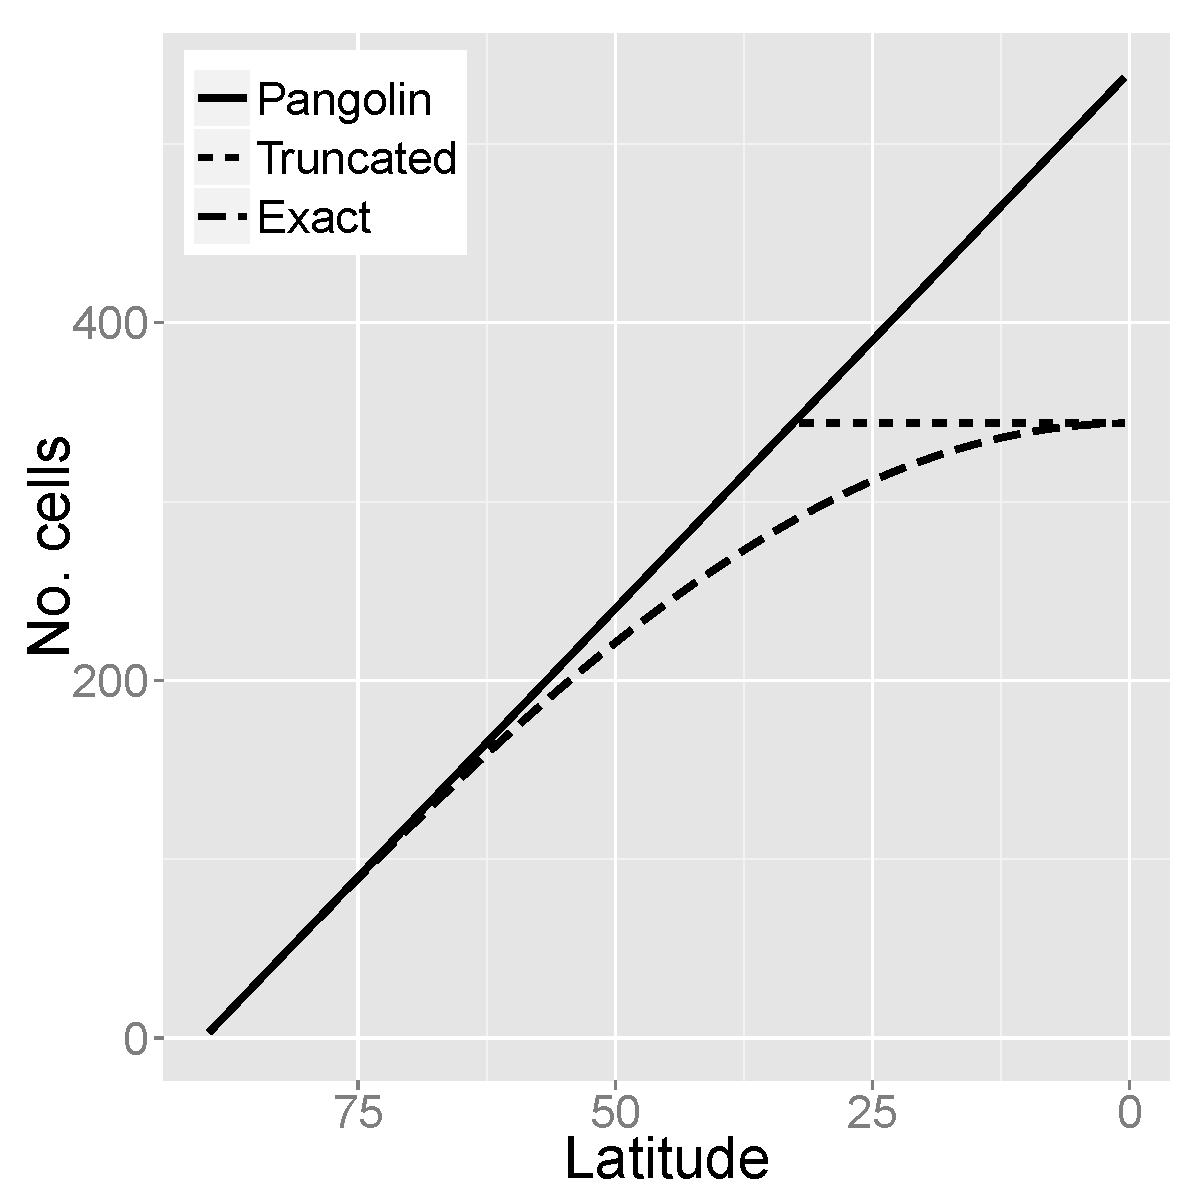
\includegraphics[width=6.5cm]{gmd-2014-119-f03.pdf}
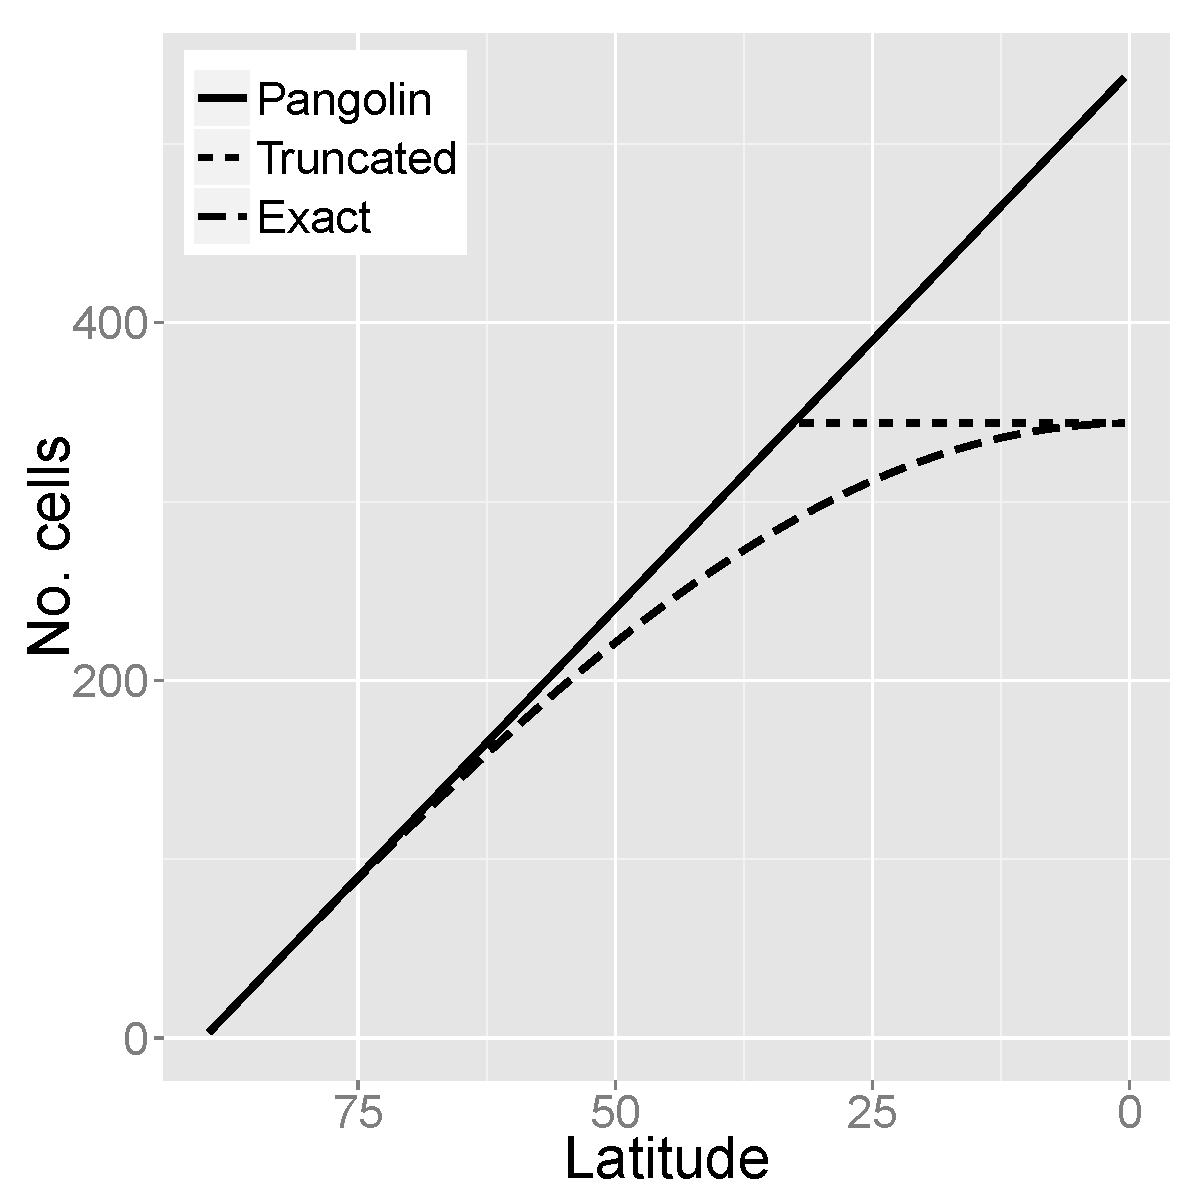
\includegraphics[width=\linewidth]{gmd-2014-119-f03.pdf}
    \caption{Number of cells for the grid used by Pangolin on one hemisphere with
      90 latitudes (solid line). The truncated and ``exact'' version are shown as
    dotted and dashed lines, respectively.}
    \label{fig2:nb_cells}%
  \end{minipage}
  \hfill
  \begin{minipage}[t]{0.48\linewidth}
    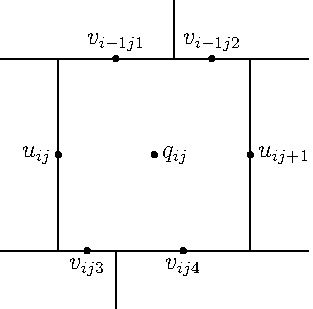
\includegraphics[width=\linewidth]{gmd-2014-119-f04.pdf}
    \caption{Discretization for zonal and meridional winds ($u$ and $v$, respectively) and tracer
    mixing ratio $q$.}
    \label{fig2:discret}%
  \end{minipage}%
\end{figure}



   The formula given in Eq.~(\ref{eqn:nb_cells2}) allows us to easily
   determine the coordinates of the cell neighbors in each zone. The
   grid used in Pangolin has four axes of symmetry -- $\lambda=0$,
   $\lambda=120$, $\lambda=240\degre$ and the Equator -- and so the grid
   can be split into six identical \textit{zones}, numbered with regard to west
   to east and north to south as shown in Fig.~\ref{fig2:pango_grid}.
   The following formulae to compute the position of the cell
   neighbors are given for the first zone -- i.e.,
   $[90\degre,0]\times[0,120\degre]$. The formulae on zones 2 and 3
   are obtained by adding the proper offset. In the Southern
   Hemisphere (zone 4 to 6), the north and south formulae are simply
   inverted. The zonal neighbors for cell $(i,j)$ are simply
   $(i,j-1)$ and $(i,j+1)$. For the first zone, its north and south
   neighbors are respectively $\big\{(i-1,j_1), \ldots, (i-1,
   j_2)\big\}$ and $\big\{(i+1,j_3), \ldots, (i+1, j_4)\big\}$,
   with
\begin{align}
&j_1 = \left\lfloor \frac{n_{i-1}}{n_i}(j-1)+1\right\rfloor,\quad
j_2 = \left\lceil \frac{n_{i-1}}{n_i}j\right\rceil,\nonumber\\
&j_3 = \left\lfloor \frac{n_{i+1}}{n_i}(j-1)+1\right\rfloor,\quad
j_4 = \left\lceil \frac{n_{i+1}}{n_i}j\right\rceil.
  \label{eqn:neighb_merid2}
   \end{align}
   From that formulation, it follows that the number of meridional
   neighbors is not constant, even though most of cells have two
   north and two south adjacent cells.  Special cases include the
   middle of each sector (one north and three south neighbors) and
   its extremities (one north and two south). These figures apply for
   the Northern Hemisphere and must be inverted in the Southern
   Hemisphere.

   As a~consequence, computing the position of the neighbors is quite
   efficient, involving mostly integer operations and roundings. These
   computations are thus performed on the fly to reduce the storage
   requirements. In a~more general way, the algebraic properties of the grid are
   exploited as much as possible. Our parallelization strategy relies heavily on the properties of the grid, as shown in Sect.~\ref{sec2:parallel}.



\subsection{Adapting the scheme to the grid}
   \label{subsec:adapting}

   For winds and tracer discretization, we adapt the Arakawa
   C grid~\citep{Arakawa1977} to our scheme, as shown in
   Fig.~\ref{fig2:discret}. To avoid interpolating the
   winds components during advection, winds are taken at the middle of
   the interfaces. Tracer concentrations are defined at the centers of
   the cells.


   Due to the structure of the grid (Fig.~\ref{fig2:pango_grid}), air and tracer
   fluxes need to be computed for all the neighbors of the cells as illustrated
   in Fig.~\ref{fig2:merid_flux}. For each flux, the frontier between the current
   cell and its neighbor is computed algebraically using the cell neighbors
   formulae (Eq.~\ref{eqn:neighb_merid2}). While there is no special treatment
   for zonal advection, meridional advection requires an interpolation to
   compute the meridional gradient. A linear interpolation in the zonal
   direction is computed to evaluate the value of the mixing ratio on the meridian
   passing through the center of the cell (see Fig.~\ref{fig2:merid_gradient}).
   These values are used to compute the meridional gradient by
   finite difference.

%f5
\begin{figure}
  \begin{minipage}[t]{0.48\linewidth}
    \centering
    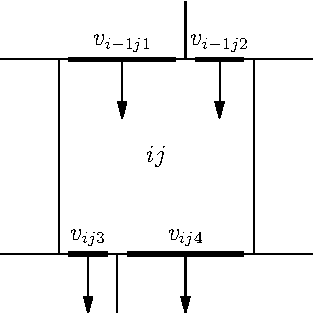
\includegraphics[width=0.8\linewidth]{gmd-2014-119-f05.pdf}
    \caption{Meridional interfaces (bold lines) and fluxes (arrows) for cell $(i,j)$.}
    \label{fig2:merid_flux}
  \end{minipage}
  \hfill
  \begin{minipage}[t]{0.48\linewidth}
    \centering
    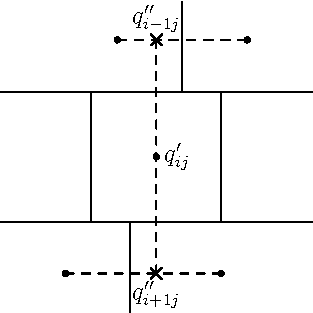
\includegraphics[width=0.8\linewidth]{gmd-2014-119-f06.pdf}
    \caption{Zonal interpolation to compute the meridional gradient of $q'_{ij}$.}
    \label{fig2:merid_gradient}
  \end{minipage}
\end{figure}



   It is critical for mass preservation that winds have a~null divergence, so we
   correct interpolated winds (both zonal and meridional) to achieve that. The
   first step in our correction deals with meridional winds. If we consider all
   the cells on a~latitude circle, the total mass variation in this ``band''
   only comes from the north and south meridional fluxes. Now, if we consider
   the latitude circle containing all south meridional fluxes, it constitutes
   a~closed contour.  Therefore, the wind divergence is null and the sum of all
   meridional winds must be zero. Meridional winds are thus corrected by
   removing the mean value from the interpolated values. For a future 3-D case, a
   preprocessing step involving vertical winds will be needed to ensure
   non-divergent circulation. Depending on the system of vertical coordinates
   used, the ``mass-winds inconsistency'' issue (see, for
   example,~\cite{Jockel2001a}) will have to be addressed.

   Then we correct zonal winds to ensure that the sum of all fluxes is
   locally null in each cell. As meridional winds are already
   corrected, only east and west zonal winds of each cell must be
   modified. We take zonal winds at longitude $0$ as a~reference and
   browse each cell sequentially from west to east to progressively correct
   each of the zonal winds and ensure mass preservation.

   Finally, we need to take care that fluxes in a~given direction do
   not completely empty the cells during an advection step. For each
   cell, a~local advective Courant number restricts the time step in order to
   avoid this situation. As advection is performed sequentially in two
   different directions, we define two uni\-dimensional local Courant
   numbers. Then the global Courant number $C$ is simply defined as
   the most restrictive condition on all cells:
\begin{align*} C = \max_{ij} \left(\frac{u_{ij}\Delta t}{\Delta\phi_{ij}},
\frac{\Delta t\sum_{k \in V_{ij}} v_k \Delta\lambda_k }{
\Delta\phi_{ij}\sum_{k \in V_{ij}} \Delta\lambda_{k}} \right),
   \end{align*}
   where $V_{ij}$ is the set of meridional neighbors for the cell
   $(i,j)$ and $\Delta\lambda_k$ is the interface size between the
   cell and its neighbor. For the tests in this paper, we use
   $C_{\text{max}}=0.96$ as a Courant–Friedrichs--Lewy~(CFL) condition.

\section{Testing suite}
   \label{sec2:tests}

   A~standard 2-D testing suite to check the accuracy and properties
   of a~transport model was proposed
   in~\citet{Lauritzen2012}. A~comparison with state-of-the-art
   schemes was subsequently published in~\citet{Lauritzen2014}, which
   offers a~convenient benchmark to compare transport models on the
   sphere.  From it, we have extracted a~subset of the models and
   cases which we felt were relevant to
   Pangolin. In~\citet{Lauritzen2014}, the different grids were
   compared with a~constant resolution at the Equator. In the present
   paper, we retain simulations performed with a~constant total number
   of cells. The number of cells in each model was computed using the
   resolution at the Equator given in the appendix
   of~\citet{Lauritzen2014}. As a~summary,
   Table~\ref{table:models_cells} contains the formulae used and
   gives an idea of the size of each grid in comparison with
   Pangolin.

%t1
\begin{table}[t]
  \centering
  \caption{For a~given resolution at the Equator, we compare the total number of
    cells of each model $n_{\text{model}}$ vs. the total number of cells of Pangolin
    $n_{\text{pangolin}}$.  }
\label{table:models_cells}
%\scalebox{.50}[.50]
{\begin{tabular}{lcc}
    \toprule
    Model & $n_{\text{model}}/n_{\text{pangolin}}$ & $n_{\text{model}}$\\
    \midrule
    FARSIGHT    & 2     & $6\cdot (90/\Delta\lambda)^2$ \\
    CLAW        & 0.68  & $2\cdot (90/\Delta\lambda)^2$ \\
    SLFV-ML     & 2.17  & NA \\
    CAM-FV      & 2.7   & $\lfloor{360/\Delta\lambda}\rfloor\cdot\lfloor{180/\Delta\lambda}\rfloor$ \\
    UCISOM      & 2.7   & $\lfloor{360/\Delta\lambda}\rfloor\cdot\lfloor{180/\Delta\lambda}\rfloor$ \\
    Pangolin    & 1   & $6\cdot{\lceil{0.5\cdot\lceil120/\Delta\lambda\rceil+1}\rceil}^2$ \\
    \bottomrule
  \end{tabular}}
\end{table}




   \subsection{Models features}

   The models were chosen as their spatial order is similar to
   Pangolin. They are implemented on both regular and non-regular
   grids and provide a~basis for a~comparison between semi-Lagrangian,
   finite-volume and wave propagation methods.  A~summary is given in
   Table~\ref{table:models}. Other features are described below:
\begin{itemize}
  \item FARSIGHT is a~grid-point semi-Lagrangian model, running on parallel
    architectures.
  \item CLAW uses a~wave propagation technique with a~first-order method
    (donor cell upwind) in each direction.
  \item SLFV-ML (Slope Limited Finite Volume scheme with Method of Lines), a~flux-form finite volume with simplified swept area and linear
    reconstruction.
  \item CAM-FV (Community Atmosphere Model
    Finite-Volume) is a~finite-volume model on a~regular latitude--longitude
    grid. It uses the piecewise parabolic method (PPM), with the addition of
    a~slope and curvature limiters.
  \item USICOM (UC Irvine Second-Order Moments scheme) is
    also a~flux-form finite volume. It uses an improved version of Prather's
    second-order moments scheme on an Eulerian regular
    latitude--longitude grid.
   \end{itemize}
   All of these models are mass preserving, so the comparison with
   Pangolin is relevant.  CAM-FV and UCISOM are of particular interest
   as they also use a~directional splitting algorithm. Furthermore,
   all models have a~shape-preserving algorithm but only FARSIGHT and
   Pangolin do not expand the initial tracer concentration range.


    \subsection{Test cases}
    \label{subsec:test_cases}

    In this paper, we only consider the case of non-divergent and
    time-dependent winds. Zonal and meridional winds ($u$ and $v$,
    respectively) are given by
\begin{align*}
  u(\lambda, \theta, t) &= \frac{10R}{T} \sin^2(\lambda')\sin(2\theta)\cos\left(\frac{\pi
  t}{T}\right) + \frac{2\pi R}{T}\cos(\theta), \\
  v(\lambda, \theta, t) &= \frac{10R}{T} \sin(2\lambda')\cos(\theta)\cos\left(\frac{\pi
  t}{T}\right),
   \end{align*}
   where $\theta$ is now the latitude and $\lambda$ the longitude,
   both in radians. $R$ is the Earth radius, $T$ is the period, set at 12~days here, and $\lambda'=\lambda-2\pi t/T$. With these winds, the
   tracer concentration first moves eastwards and is then deformed
   into filaments up to $t=T/2$. After that, the flux is inverted and
   the tracer continues to move to the east until it comes back to its
   initial distribution at $t=T$.

   These winds provide an easy way to compute the errors as the
   solution after a~full period can be simply compared with the
   initial concentration. We will use the same normalized errors as
   in~\citet{Lauritzen2012}:
\begin{equation*}
  \ell_2(q) = \sqrt{\frac{\mathcal{I}((q-q_0)^2)}{\mathcal{I}(q_0^2)}}
  \quad \text{and} \quad
  \ell_{\infty}(q) = \frac{\displaystyle\max_{\forall\lambda, \theta}{|q - q_0|}}{\displaystyle\max_{\forall\lambda, \theta} |q_0|},
   \end{equation*}
   where $q=q(\lambda,\theta,t)$ is the tracer concentration and $q_0$
   the initial concentration.  Also, $\mathcal{I}$ is defined as the
   global integral:
\begin{equation*}
  \mathcal{I}(q) =
  \frac{1}{4\pi}\int_{0}^{2\pi}\int_{-\pi/2}^{\pi/2}{q(\lambda,\theta,t)\cos\theta
  \mathrm{d}\lambda \mathrm{d}\theta}.
    \end{equation*}

    For our model, the tracer mixing ratio is approximated as linear
    functions in a~cell. Thus the mean value corresponds to the
    value at the middle of the cell, so the integral is approximated
    by $\mathcal{I}(q) = \sum_{i,j}{\widehat{q}_{ij}} \mathcal{A}_{ij}$, where
    $\widehat{q}_{ij}$ is the tracer mean value in cell $(i,j)$ and
    $\mathcal{A}_{ij}$ its area given by Eq.~(\ref{eqn:cell_area}).

Two initial conditions are used here: a sum of two Gaussian hills and a sum of two cosine bells.
We note $(\lambda_1,\theta_1)=(5\pi/6,0)$ and
$(\lambda_2,\theta_2)=(7\pi/6,0)$ as the coordinates of the two ``centers'' used
below. Gaussian hills are defined as
\begin{equation*}
  q(\lambda, \theta) = h_1(\lambda, \theta) + h_2(\lambda, \theta).
\end{equation*}

Noting $h_{\text{max}}=0.95$ and $b=5$, for $i=1,2$ we have
\begin{equation*}
 h_i(\lambda, \theta) =
 h_{\text{max}} e^{-b((X-X_i)^2+(Y-Y_i)^2+(Z-Z_i)^2)},
   \end{equation*}
   where $X,Y,Z$ are the Cartesian coordinates of $(\lambda, \theta)$
   and $X_i,Y_i,Z_i$ are the Cartesian coordinates of $(\lambda_i,
   \theta_i)$ for~${i=1,2}$.  Cosine bells are defined by
\begin{equation*}
  q(\lambda, \theta) =
  \begin{cases}
    b + c\times h_1(\lambda, \theta) \quad \text{if} \quad r_1 < r,\\
    b + c\times h_2(\lambda, \theta) \quad \text{if} \quad r_2 < r,\\
    b \quad \text{otherwise,}
  \end{cases}
   \end{equation*}
   with the background value $b=0.1$ and amplitude $c=0.9$. Noting
   $h_{\text{max}}=1$ and $r=R/2$, we also have
\begin{equation*}
  \forall i=1,2, \quad h_i(\lambda, \theta) =
  \displaystyle\frac{h_{\text{max}}}{2}\left(1+\cos\left(\pi\frac{r_i}{r}\right)\right),
\end{equation*}
where the $r_i$ are the great-circle distances to $(\lambda_i,\theta_i)$ on the
sphere:
\begin{equation*}
  r_i(\lambda, \theta)=R \arccos(\sin\theta_i\sin\theta +
  \cos\theta_i\cos(\lambda-\lambda_i)).
\end{equation*}

   Pangolin results for the Gaussian hills and cosine bells test cases
   are shown in Fig.~\ref{fig2:gaussianT2} at $t=0$, half the period
   and after a~full period.  The shape of the tracer distribution
   is well preserved but numerical diffusion contributes to a decrease in
   the tracer maxima, as it appears at $t=T/2$ and $t=T$. To compute the
   numerical order of convergence in Sect.~\ref{subsec:conv}, results at $t=0$ and
   $t=T$ will be used, while the preservation of filaments in
   Sect.~\ref{subsec:preserv} is computed using the results at $t=0$
   and $t=T/2$.
%t2
\begin{table*}[t]
  \caption{Summary of the models used as a~comparison: name, implementation
  grid, the total number of cells vs. Pangolin, and the time scheme.}
%\scalebox{.750}[.750]
{\begin{tabular}{llcll}
    \toprule
    Model & Grid & Formal  & Time & Reference \\
     &  &  accuracy &  scheme &  \\
    \midrule
    FARSIGHT    & Gnomonic cubed sphere &  2 & Third order & \citet{White2011} \\
    CLAW        & Two-patch sphere grid &  2 & Euler forward &
    \citet{LeVeque2002} \\
    SLFV-ML     & Icosahedral--hexagonal &  2 & Runge--Kutta 3rd-order TVD &
    \citet{Miura2007} \\
    CAM-FV      & Regular lat--long       &  2 & Euler forward & \citet{Collins2004}\\
    UCISOM      & Regular lat--long       &  2 & Euler forward & \citet{Prather1986} \\
    Pangolin    & Pangolin              &  2 & Euler forward & This paper \\
    \bottomrule
  \end{tabular}}
\label{table:models}
\end{table*}



%f7
\begin{figure*}[t]
  \centering
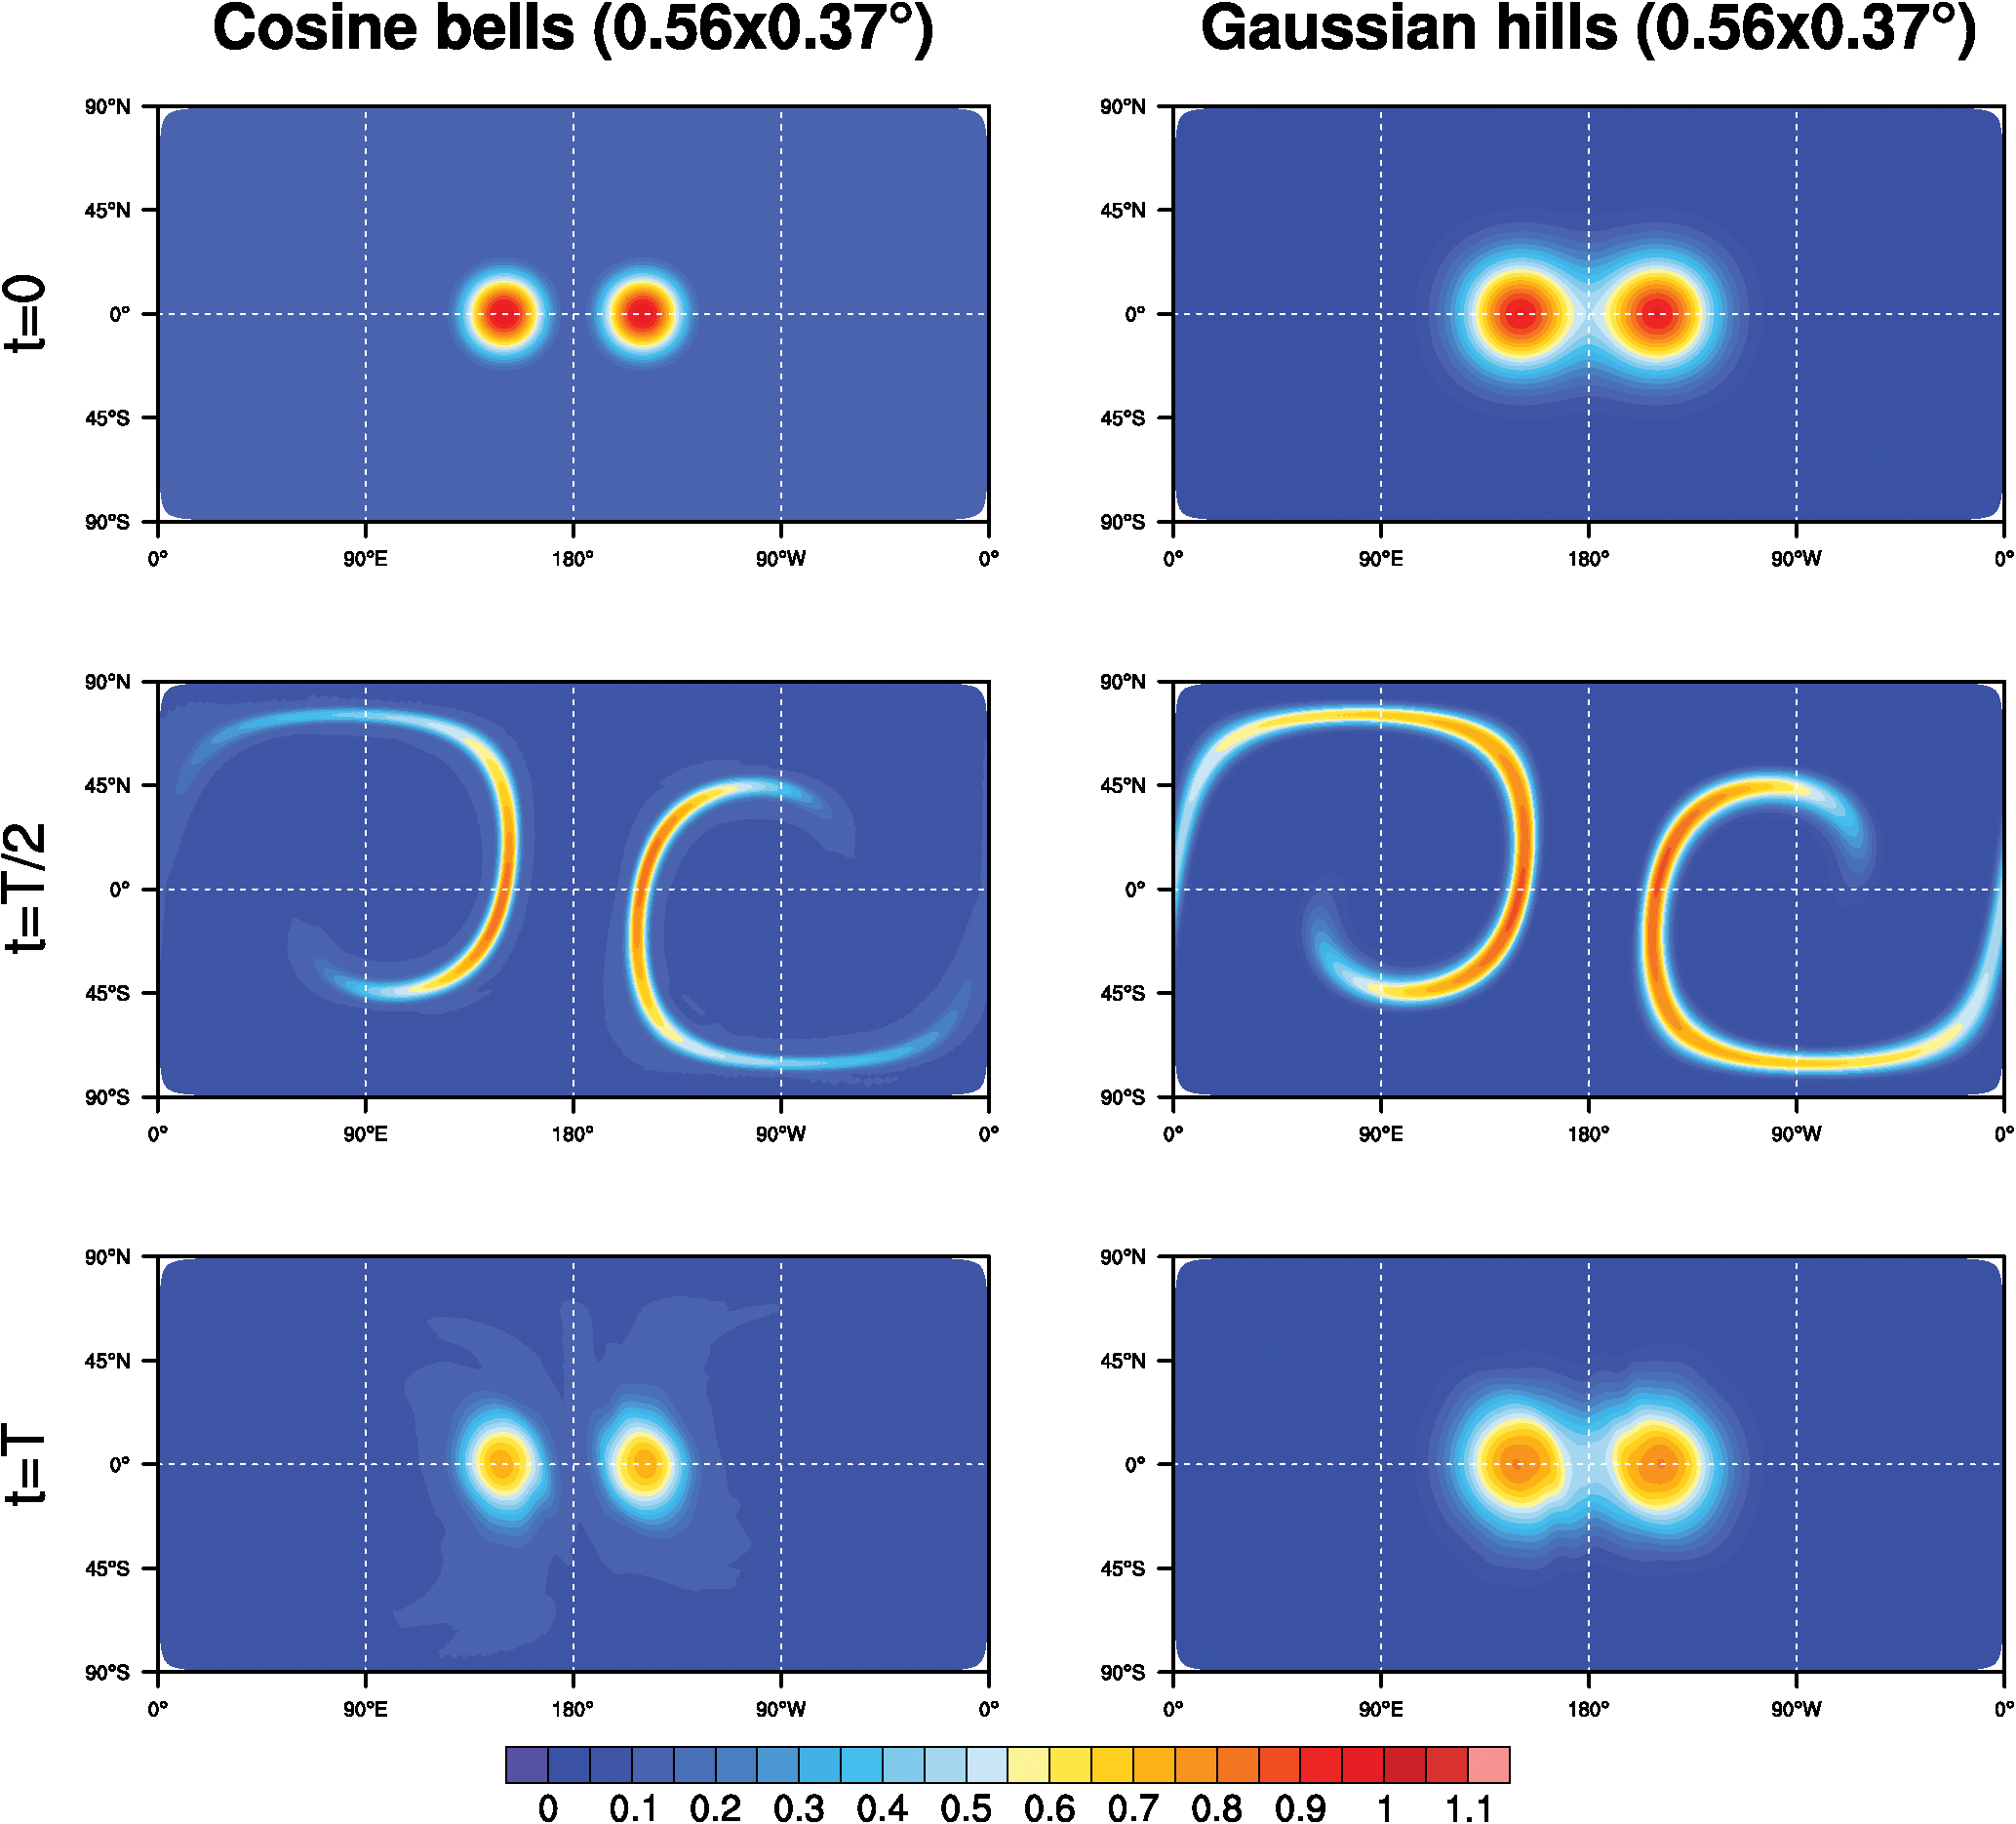
\includegraphics[width=11.5cm]{gmd-2014-119-f07.png}
\caption{Cosine bells and Gaussian hills results for $t=0$, $t=T/2$, $t=T$
    (top to bottom) with Pangolin. The initial distribution is first deformed
    into filaments and then advected back to its initial position. The Equator
    resolution is $0.56{\degre}\times0.37\degre$.  For these plots, Pangolin data
    are interpolated to a~regular latitude--longitude grid.}
\label{fig2:gaussianT2}
\end{figure*}



\subsection{Numerical order of convergence}
   \label{subsec:conv}

   The aim of this test is to check the rate at which numerical error decreases
   when resolution increases. Ideally, this rate should be close to
   the theoretical order of convergence. The Gaussian hills test case is
   used here, as it provides an infinitely smooth function. Results
   are plotted in Fig.~\ref{fig2:cv_rate}, where $\ell_2$ and
   $\ell_{\infty}$ are plotted with a~varying number of cells.  When
   available, the impact of shape-preserving filters is also
   represented on the plot, with the exception of UCISOM. For this
   choice of models, it does not reduce errors in a~significant way as
   can be expected from lower-order models.

%f8
\begin{figure*}[t]
  \centering
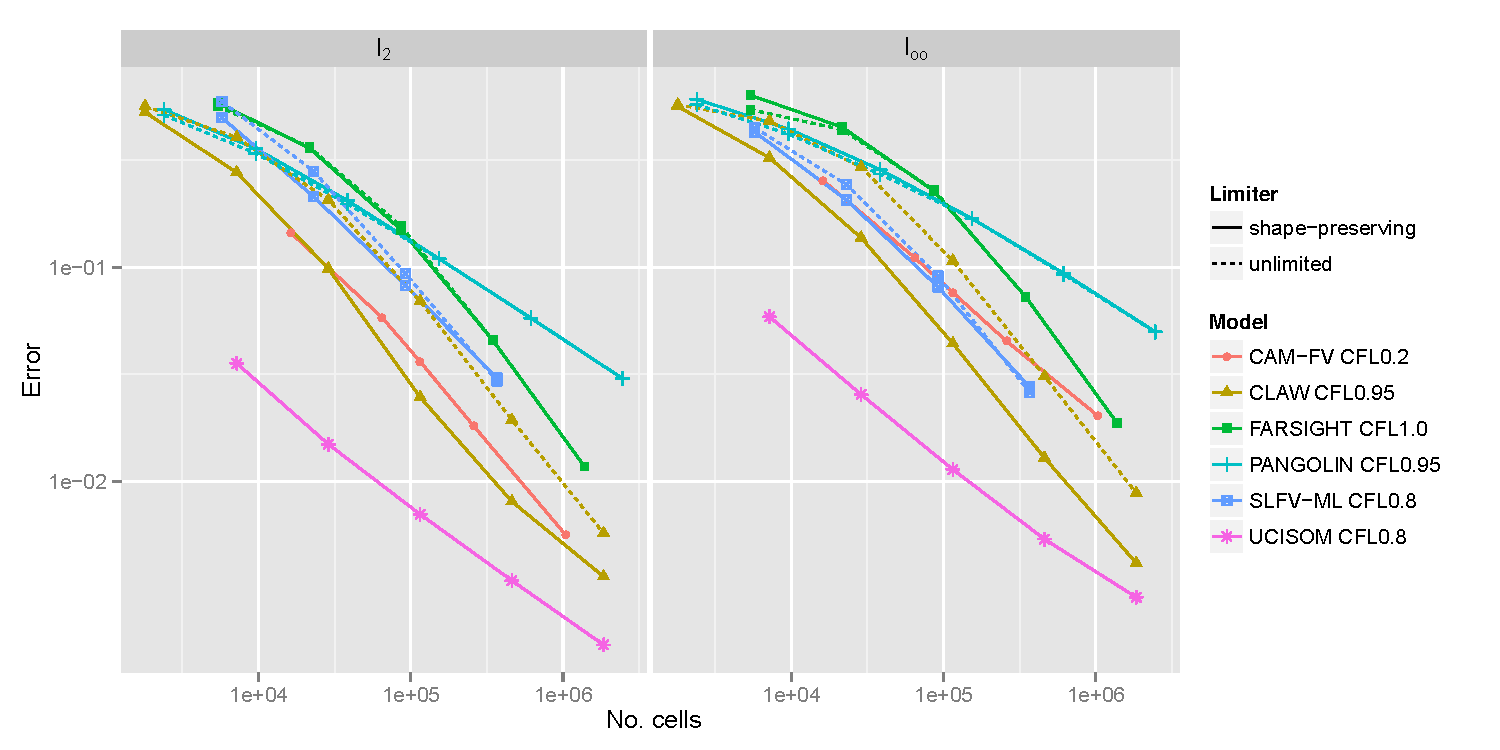
\includegraphics[width=12cm]{gmd-2014-119-f08.pdf}
\caption{Numerical order of convergence for both error measures. These are computed using
  Gaussian hills after a~full rotation. When available, the models are shown
  with and without the shape-preserving limiters.}
\label{fig2:cv_rate}
\end{figure*}



   For errors at low and medium resolutions, Pangolin is quite close to
   the other models, with the exception of UCISOM. However, the errors
   with a~large number of cells are lower for models other than
   Pangolin. One possible explanation is the loss of accuracy due to
   the interpolation when computing the meridional gradient. In
   general, the order of convergence of Pangolin is lower. To quantify
   that, we use numerical optimal order of convergences corresponding to
   the errors $\ell_2$ and $\ell_{\infty}$. They result from
   a~least-squares linear regression on the errors plotted vs. the
   resolution at the Equator:
\begin{equation*}
  \log(\ell_i) = -\kappa_i \log(\Delta\lambda) + b_i
  \quad \text{with} \quad i=2,\infty.
   \end{equation*}

   For Pangolin, the regression is applied after the optimal
   convergence has been reached. This corresponds to longitudinal
   resolutions at the Equator in the range
   $[0.75\degre,0.1875\degre]$. The final numerical convergence
   rates are shown in Fig.~\ref{fig2:num_cv_rate}.

   This selection of models and parameters shows that theoretical order
   is not achieved for all models. For most of them, using a~different
   Courant number does not improve the convergence speedup, with the
   exception of FARSIGHT and CAM-FV.  Using a~Courant number of 10.4 (1.2)
   greatly improves the result of FARSIGHT (CAM-FV) with a~Courant
   number of 1.4 (0.2).


%f9
\begin{figure*}[t]
  \centering
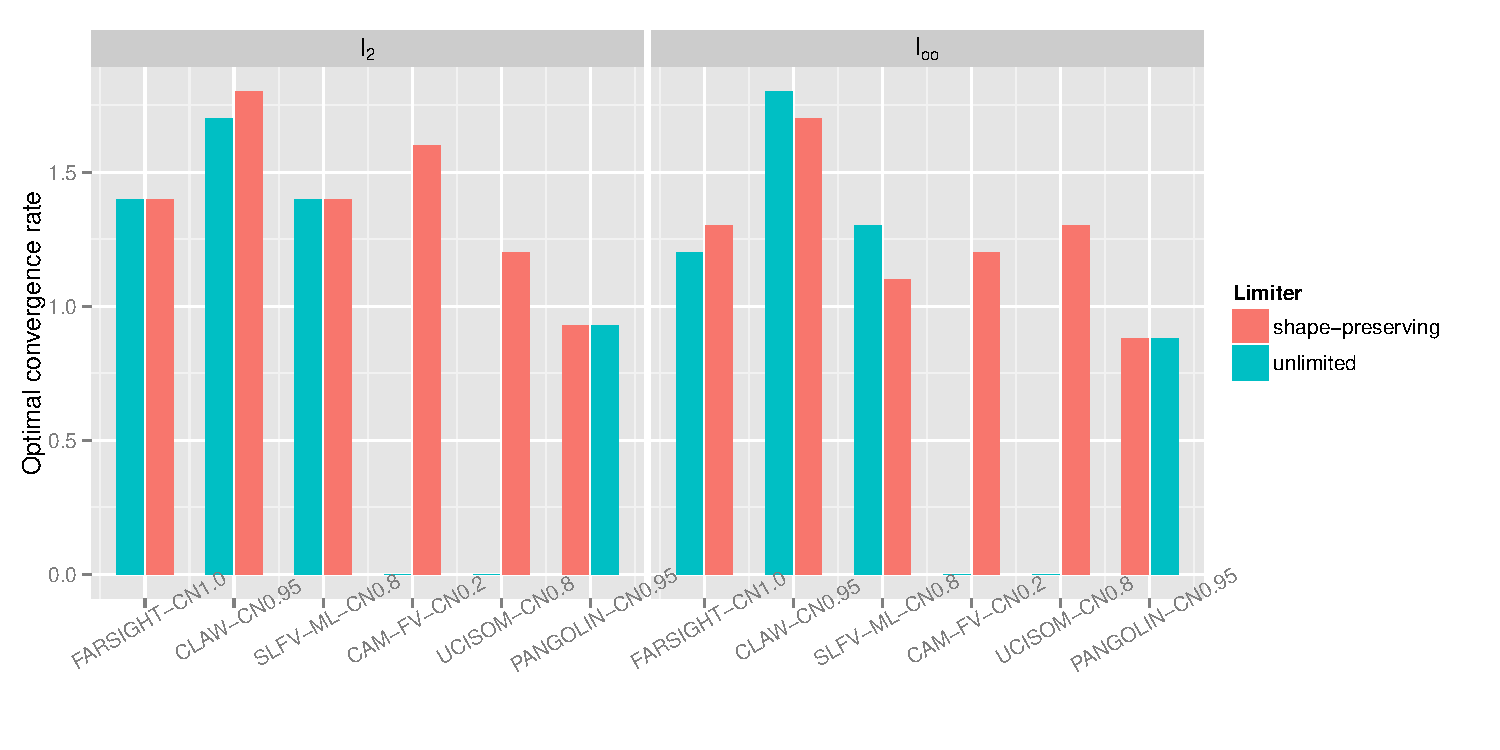
\includegraphics[width=10cm]{gmd-2014-119-f09.pdf}
\caption{Optimal order of convergence computed by a~least-squares regression on
    data from Fig.~\ref{fig2:cv_rate}. Some models did not offer data without
  shape-preserving limiters (CAM-FV, UCISOM).}
\label{fig2:num_cv_rate}
\end{figure*}



   Furthermore, we can see the numerical order of convergence of Pangolin is
   lower than other models. This is not surprising when comparing with similar
   finite-volume schemes such as CAM-FV and UCISOM, which use higher-order schemes in
   one or more directions. We studied this issue further using solid-body
   rotation test cases (described in~\cite{Williamson1992}) and found that the
   accuracy was limited by the linear interpolation done for the meridional
   gradient. When the axis of the solid-body rotation matches the polar axis,
   accuracy is close to second order, whereas the level of accuracy decreases
   when the axis is in the equatorial plane. In practice, Pangolin needs finer
   resolutions, as shown in the following test cases, to match the accuracy of
   other models.

%f10
\begin{figure*}[t]
  \centering
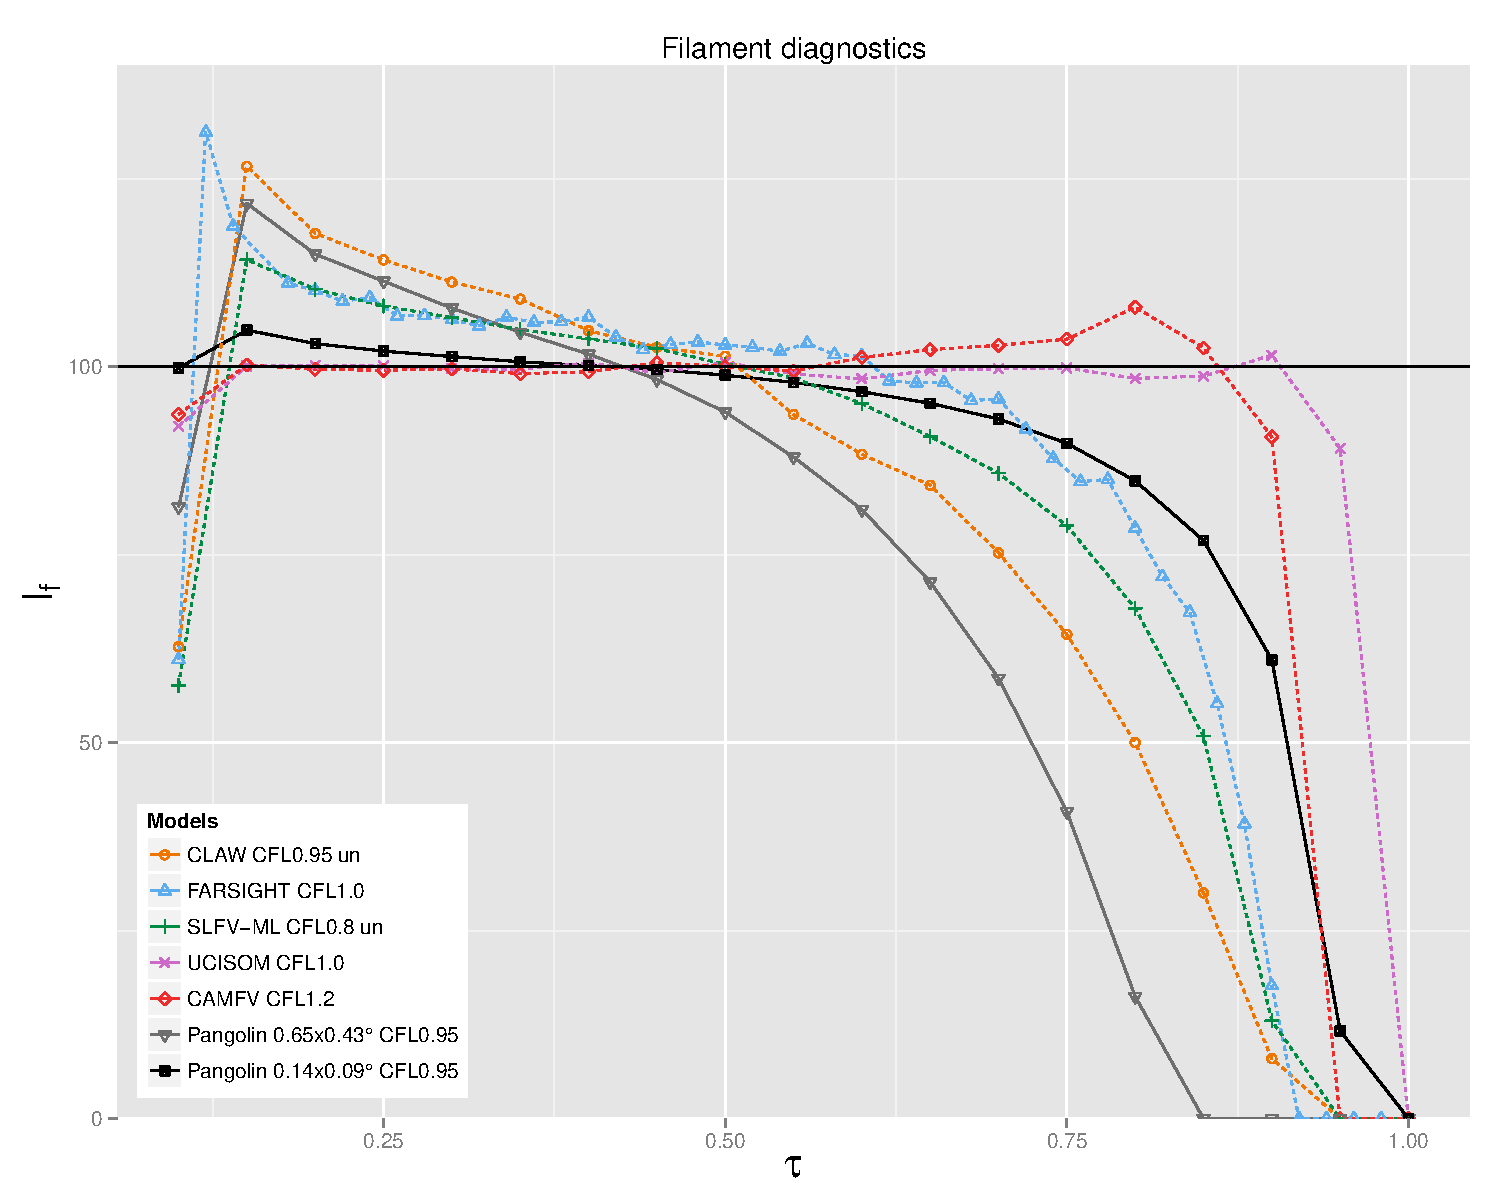
\includegraphics[width=12cm]{gmd-2014-119-f10.pdf}
\caption{Filament diagnostics between for Pangolin (solid line) and other
  models (dashed line).  By default, the shape-preserving version is used. Only
CLAW and SLFV-ML use an ``unlimited'' version.}
\label{fig2:filaments}
\end{figure*}

\subsection{Preservation of filaments}
   \label{subsec:preserv}

   Realistic distributions will most likely be deformed into filaments when the
   tracer material is stretched and gradients are increased. For some
   applications, it is important to check how well these filaments are
   preserved. In the cosine bells test case, the initial concentration is
   deformed into thin filaments up to $t=T/2$, before being advected to the
   initial position. Diagnostics are thus computed at $T/2$.

   Let us consider the area where the tracer is greater than a~given
   threshold $\tau$. For non-divergent flows and for all thresholds, if this
   area is not preserved at all times, it suggests filaments are
   degraded. This leads to the definition of the following diagnostic:
\begin{align*}
  \ell_{\mathrm{f}} =
    \begin{cases}
      \displaystyle 100 \times \frac{A(\tau,t)}{A(\tau,0)} \quad \text{if} \;
      A(\tau,0) \neq 0,\\
      0 \quad \text{otherwise,}
    \end{cases}
    \end{align*}
    where $A(\tau,t)$ is the surface area for which the tracer ratio
    at time $t$ is greater or equal to $\tau$. For Pangolin and other
    Eulerian schemes, $A(\tau,t)$ is defined as the sum of the cell
    areas where $q(t) \ge \tau$.  Thus the closest $\ell_{\mathrm{f}}$ is to
    $100$, the better the filaments are preserved.


  %f11
\begin{figure}[t]
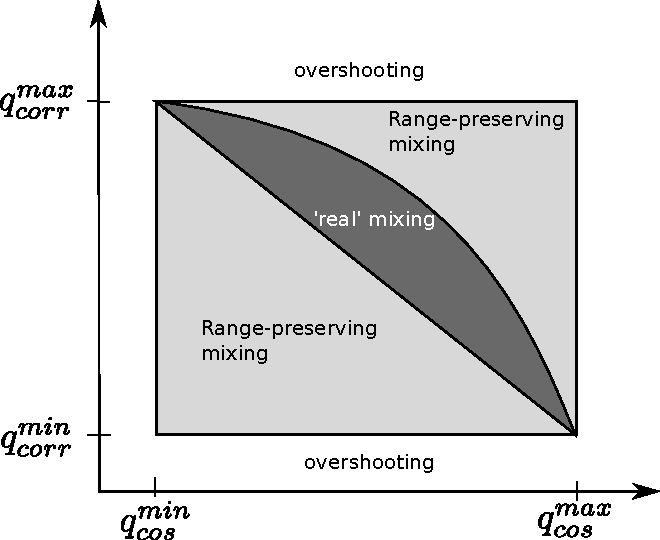
\includegraphics[width=7.5cm]{gmd-2014-119-f11.pdf}
  \centering
\caption{Different types of mixing when plotting the correlated concentration
  against the cosine bells distribution.}
\label{fig2:mixing}%
\end{figure}%

    Results are shown in Fig.~\ref{fig2:filaments}. All models except Pangolin
    are compared with different numbers of cells but with the same resolution of
    0.75{\degree} at the Equator. Pangolin is shown with two different numbers of
    cells. The first case (shown as grey solid line) has a~resolution of
    approximately 0.75{\degree} at the Equator. The second one (shown as
    black solid line) is a~higher-resolution version (0.1{\degree} at the Equator)
    which approaches the results of more accurate models.

    The behavior of the models on non-latitude--longitude grids (all
    models except UCISOM and CAM-FV) is typical of diffusive
    schemes. They tend to diffuse the base of the distribution and
    reduce the maxima, thus leading to an increase in $\ell_{\mathrm{f}}$ for
    small $\tau$ and a~decrease in $\ell_{\mathrm{f}}$ for large $\tau$.
    Another piece of information we can extract from this is the alteration of
    gradients. Here CAM-FV can be seen to have $\ell_{\mathrm{f}} > 100$ for
    large $\tau$, which results from gradient steepening. On the
    other hand, schemes on non-regular grids have a~smooth and
    decreasing profile, showing that the scheme diffusion is also smooth
    and continuous.


%f12
\begin{figure}[t]
  \hspace*{-0.3cm}
  \begin{minipage}[t]{0.5\linewidth}
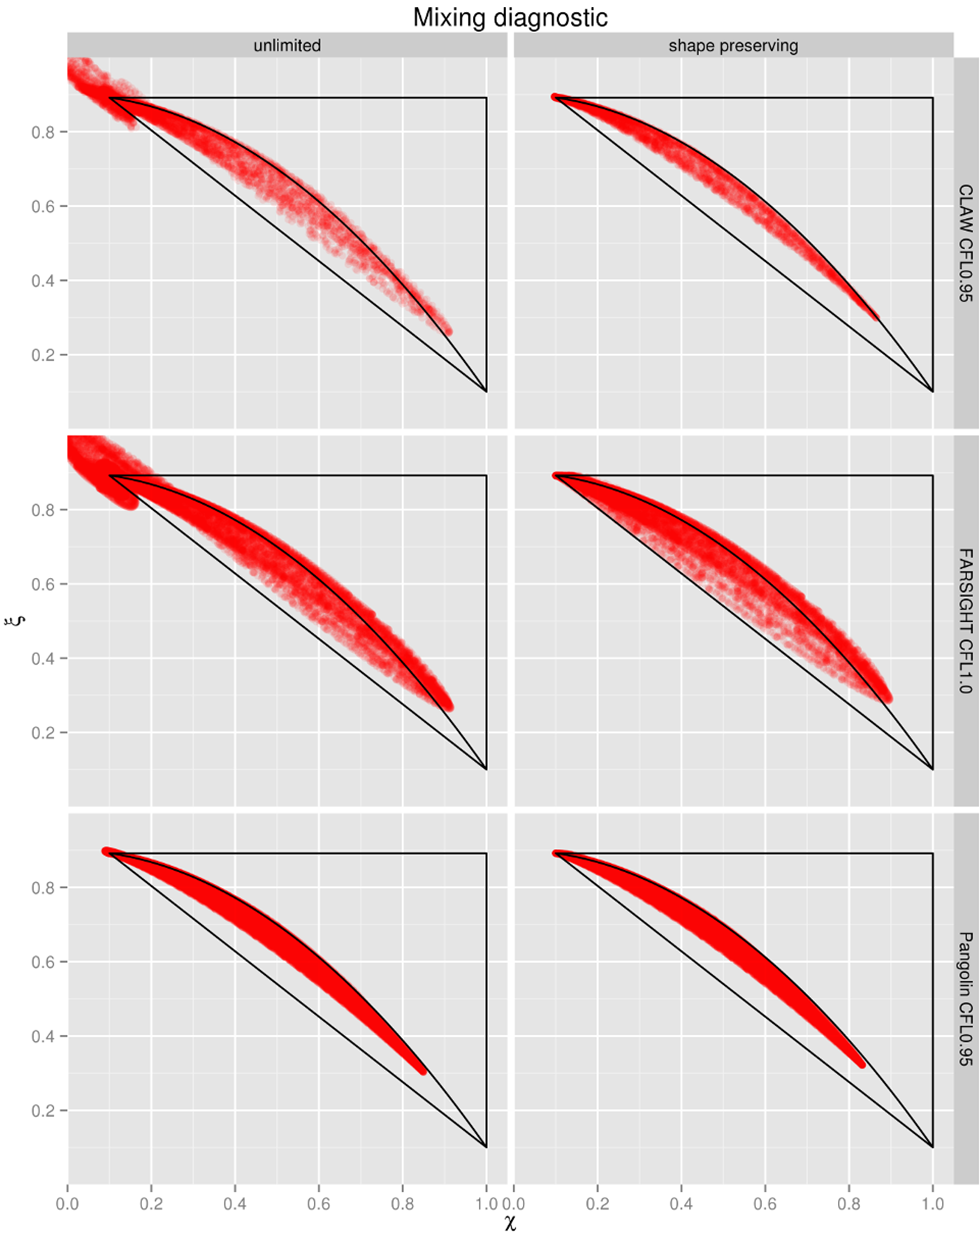
\includegraphics[width=\linewidth]{gmd-2014-119-f12.png}
  \end{minipage}
  \begin{minipage}[t]{0.5\linewidth}
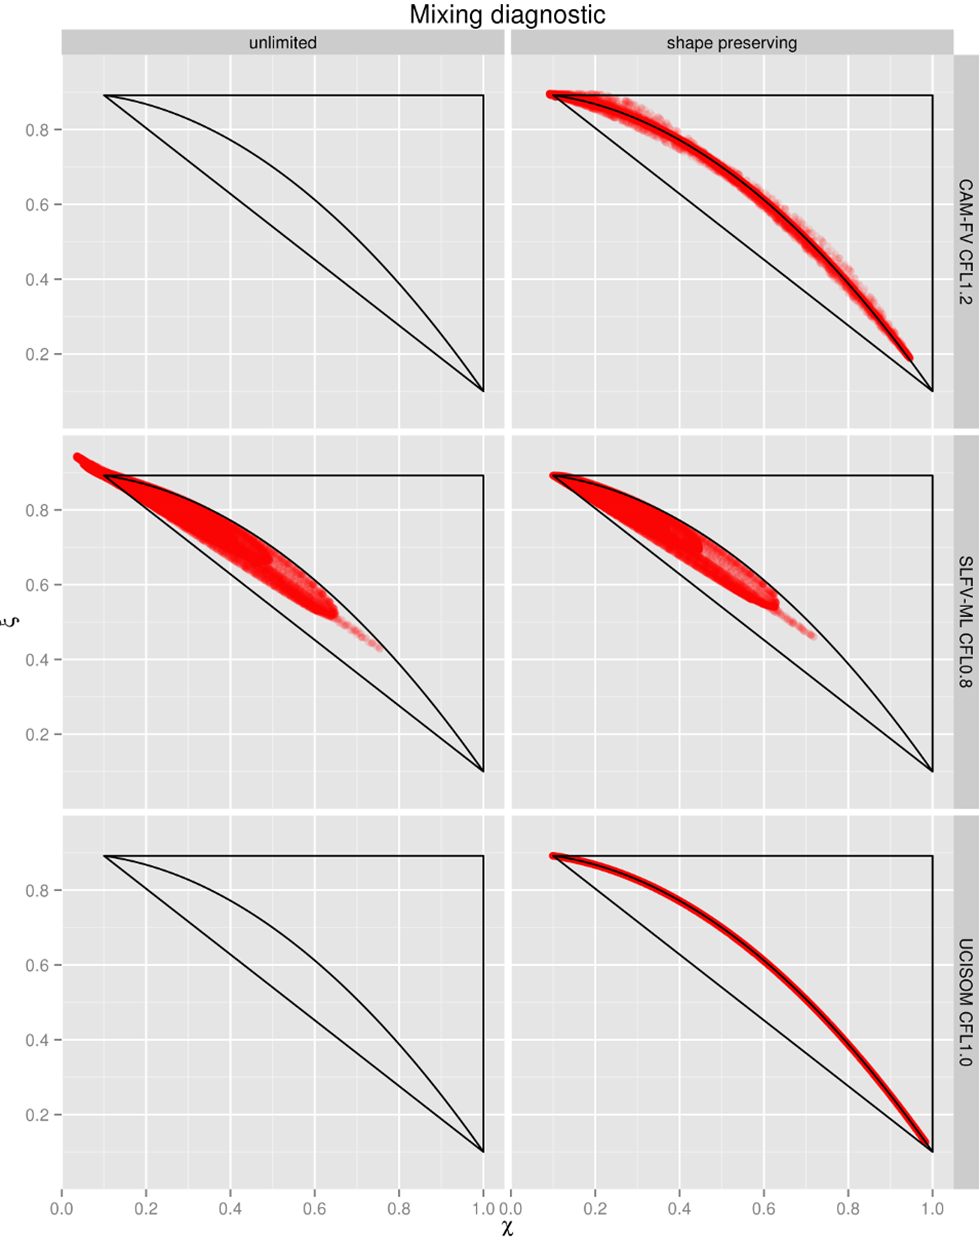
\includegraphics[width=\linewidth]{gmd-2014-119-f13.png}
  \end{minipage}
\caption{Mixing plots for both unlimited and shape-preserving versions.
    The resolution is set at $0.75\degre$ at the Equator, except for Pangolin,
  which has $0.376\degre$.}
\label{fig2:mixing1}%

\end{figure}%

    Furthermore, the shape from the diagnostic for Pangolin is quite close to
    models using non-regular latitude--longitude grids (CLAW, FARSIGHT, SLFV-ML).
    The behavior is typical of diffusive schemes, where $\ell_{\mathrm{f}}$ is
    increased for lower threshold values and decreased for higher $\tau$.
    Pangolin is less accurate than these models, but similar accuracy can be
    achieved using a finer resolution. Nevertheless, the models using a regular
    latitude--longitude grid, namely UCISOM and CAM-FV, are the most accurate for
    this test.

      \subsection{Preservation of preexisting relations}

   When advecting several correlated tracers, numerical transport
   schemes should preserve the relations between them.  However,
   errors due to numerical diffusion can modify these relations and
   introduce a ``mixing''.  This is by no means an unphysical feature
   as real-life tracers can undergo some mixing too, either by
   chemical reactions or diffusion. This test aims at assessing the
   amount of unphysical mixing. To that end, we
   follow~\citet{Lauritzen2012} and use a~first tracer with the cosine
   bells initial condition $q_{\text{cos}}(t=0)$ and a~second tracer
   correlated to the first:
\begin{align}
&q_{\text{corr}}(t=0) = -0.8 q_{\text{cos}}^2(t=0) + 0.9.
  \label{eqn:corr}
  \end{align}

  After a~half-period of advection using the non-divergent winds for
  each case, we plot $q_{\text{corr}}(t=T/2)$ against
  $q_{\text{cos}}(t=T/2)$ as a~scatterplot. Depending on the position
  of the points, we can then check the mixing level. An illustration
  of the different zones is given in Fig.~\ref{fig2:mixing}.  The
  shaded convex area in the figure corresponds to ``real''
  mixing as it contains all the lines between two points on the curve
  corresponding to Eq.~(\ref{eqn:corr}). The light-grey area is not a~physical mixing
  but is still in the initial range.  Everything outside the box is
  overshooting, which may result in unphysical concentrations such as negative
  values.




  Results are shown in Fig.~\ref{fig2:mixing1}. All unlimited schemes present some overshooting
  in the upper left corner of the figure, which is then removed with
  a~shape-preserving filter. Also, all schemes, with the exception of
  UCISOM, present real mixing. For this selection of models, only
  FARSIGHT and CAM-FV have range-preserving unmixing. For FARSIGHT,
  this can be removed with a~larger Courant number. In that case, its accuracy
  is on the same level as UCISOM.  Concerning accuracy, the closer the points
  lie to the curved defined in Eq.~(\ref{eqn:corr}), the more the scheme
  preserves the initial relation. In that respect, UCISOM is the most accurate
  model of this selection, followed by Pangolin and CAM-FV.

  \subsection{Comparing parallel performances}

  Pangolin was designed with scalability and parallel performances in mind, thus
  leading to the choice a smaller stencil than the models presented here.  From
  the results presented above, it is clear Pangolin can match the accuracy of
  other models using finer resolution. Unfortunately, comparing the parallel
  performances in terms of running time on multi-core architectures is difficult. Some
  models provide technical details about the performances --
  see~\cite{White2011} for FARSIGHT, \cite{Dennis2011} for CAM-FV or
  \citet{Erath2014} and \citet{Guba2014} for some other state-of-the art schemes -- but
  there are not enough data for a thorough comparison. We thus provide
  as much detail as possible on the parallel performances of Pangolin alone. In
  particular, Sect.~\ref{subsec:performances} highlights the smallest size of
  subdomains needed for a reasonable efficiency for 2-D parallel advection.

\section{Parallelization}
   \label{sec2:parallel}



   For large-scale numerical simulations, using only sequential computations is
   no longer affordable. To use a~parallel approach, we need to split and
   balance the computational effort among a~set of computing units.  For partial
   different equation-based simulations where the computational cost is evenly
   shared among the cells, a~natural and widely used approach is to partition
   the computational domain into connex subdomains of similar sizes. Each
   subdomain is handled by a~different computing unit that leads a~well-balanced
   parallel calculation.

   The original objectives in designing this model were
   twofold. First, we intended to have a~discretization with cells of
   equal areas so that the CFL condition is not penalized by the
   smallest cells. Second, we targeted a~semi-structured grid to avoid
   managing complex data structures, as well as an extra-tool to
   generate it. This leads us to define the grid detailed in
   Sect.~\ref{subsec:grid}, where computing the neighbors of grid
   cells is fully algebraic. In a~parallel framework, this grid has an
   additional asset as it enables a custom algebraic
   partitioning. Otherwise, mesh splitting often requires
   sophisticated mesh partitioning tools such as those developed
   by~\citet{Karypis1995} and \citet{Pellegrini2012}.

   \subsection{Partitioning}

   In order to perform the partitioning, we first exploit the grid
   symmetries. The grid is composed of six identical zones as
   described in Sect.~\ref{subsec:grid}.  We then focus on
   partitioning one of these zones, which contains $n^2_\mathrm{lat}$ cells, where
   $n_\mathrm{lat}$ is the number of latitudes in the hemisphere. A~perfect work
   balance occurs when there are $p^2$ subdomains with $p$ dividing
   $n_\mathrm{lat}$. In this case, each subdomain contains exactly $(n_\mathrm{lat}/p)^2$ cells.
   The most natural way to gather cells to form the subdomains is to
   use the same algorithm as the one to build the grid. The $p^2$
   subdomains are set on $p$ bands, where the $k$th band contains
   $2k-1$ subdomains ($k>0$). Applying the same decomposition to the
   remaining five zones leads to the structure shown in
   Fig.~\ref{fig2:partitioning}.

%f14
\begin{figure}[t]
  \centering
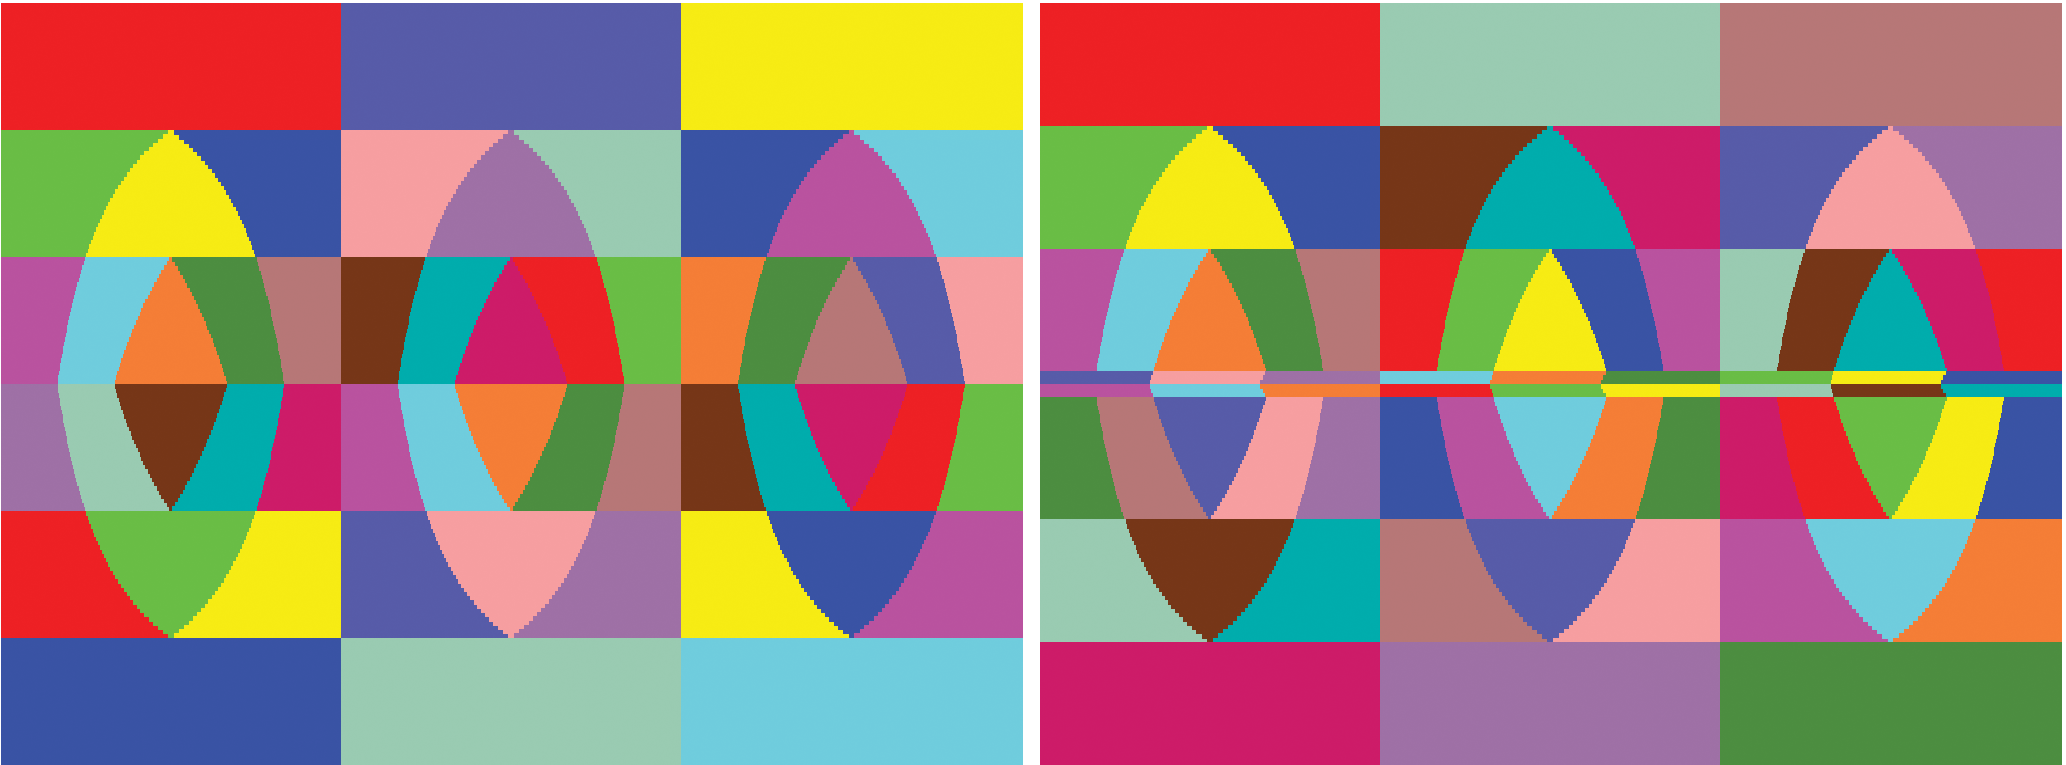
\includegraphics[width=8.5cm, height=4cm]{gmd-2014-119-f14.png}
  \caption{Algebraic mesh partitioning for an optimal case (54 domains, left) and
    sub-optimal case (74 partitions, left). Each color corresponds to a~subdomain (the
    same color can be used for different subdomains). The grid contains 48\,600~cells and is shown in latitude--longitude coordinates. }
  \label{fig2:partitioning}%
\end{figure}%





   For the sake of flexibility, this optimal situation can be slightly
   degenerated to accommodate any number of subdomains. For these
   sub-optimal situations, we consider the closest lower square $p'^2$
   on a~zone, with $p'$ dividing $n_\mathrm{lat}$.  These $p'^2$ subdomains are set
   according to the previous strategy. The remaining $p^2-p'^2$ cores
   are associated with on a~special band, with less cells and thus
   without preserving the partition size.

   These results are given for one zone only. For the complete grid,
   we find the optimal number of subdomains is $6p^2$ with $p$
   dividing $n_\mathrm{lat}$. Otherwise, the model can manage any number of
   subdomains on one-third of the grid (between longitude 0 and
   120). The total number of subdomains in these optimal cases is then
   a~multiple of 3.  It is worth noting that~\citet{White2011}
   need a~condition similar to our perfect case for their parallel
   version: the number of subdomains must be of the form $6p^2$, with
   $p$ dividing the number of cells on a~cube edge.

   This algebraic partitioning uses the regular topology of the grid to create
   subdomains with a~regular shape. This feature ensures regular data access and
   allows for possible optimizations by anticipation strategies such as
   pre-fetching to improve faster data access by loading data into the cache
   before it is actually needed. To highlight this regularity, and for the sake
   of comparison, we display in Fig.~\ref{fig2:scotch} the partition computed by
   the mesh partitioner Scotch~\citep{Pellegrini2012} for the same grid as in
   Fig.~\ref{fig2:partitioning}. One can observe that this general-purpose tool
   does not succeed in preserving the regular shape of the subdomains. In
   addition, our partitioning reduces the number of neighbors for the
   subdomains and consequently the number of messages exchanged. The total
   number of neighbors of our partitioning is divided by at least 2 when
   compared with Scotch, even in sub-optimal cases.

%f15
\begin{figure}[t]
  \centering
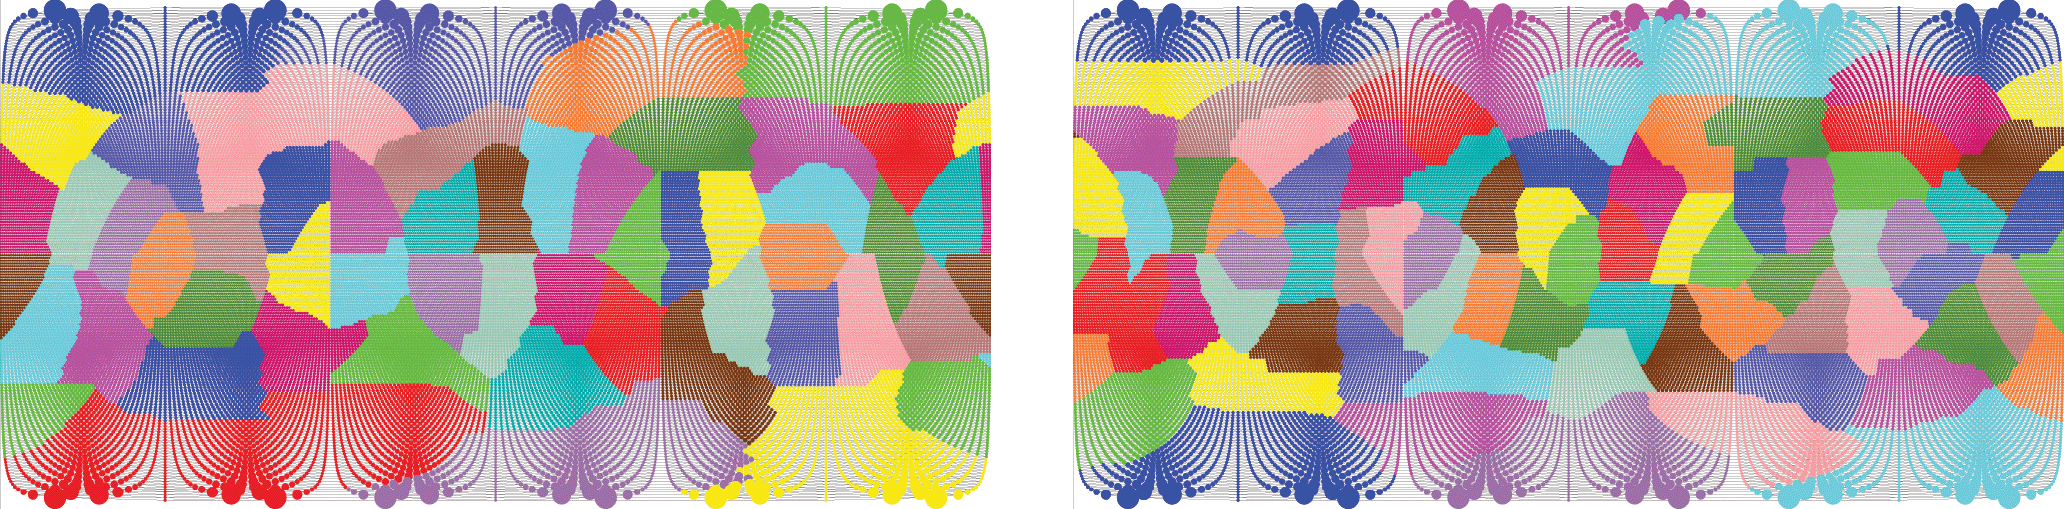
\includegraphics[width=8.5cm, height=4cm]{gmd-2014-119-f15.png}
  \caption{Mesh partitioning computed by the general purpose mesh partitioner
    Scotch for 54 domains (optimal case for Pangolin, left) and 72 domains
    (sub-optimal case for Pangolin, right). Each color corresponds to a~subdomain
    (the same color can be used for different partitions). The grid contains
  48\,600~cells and is shown in latitude--longitude coordinates.  }
  \label{fig2:scotch}%
\end{figure}%


   \subsection{Parallel implementation}

   Our parallel implementation first targets distributed memory
   architectures.  Therefore, we consider a~message passing parallel
   implementation on top of the MPI library where each subdomain is
   assigned to a~different computing unit.  To update the tracer ratio
   for all the cells in a~subdomain, most of the information required
   to compute the fluxes is already available in the subdomain.
   However, some communications need to be performed to exchange
   information along the interfaces generated by the partitioning. For
   example, zonal fluxes need to exchange concentration and gradient
   data with the east and west neighboring subdomains. In that
   respect, we introduce ghost cells which store data received
   from the neighbors via message exchanges. It should be noted that,
   due to the shape of the subdomains, meridional advection requires
   communications with the north, south, east and west
   neighbors. This is illustrated in Fig.~\ref{fig2:ghost_cells},
   where the ghost cells are shown as hatched cells.


%f16
\begin{figure}[t]
  \centering
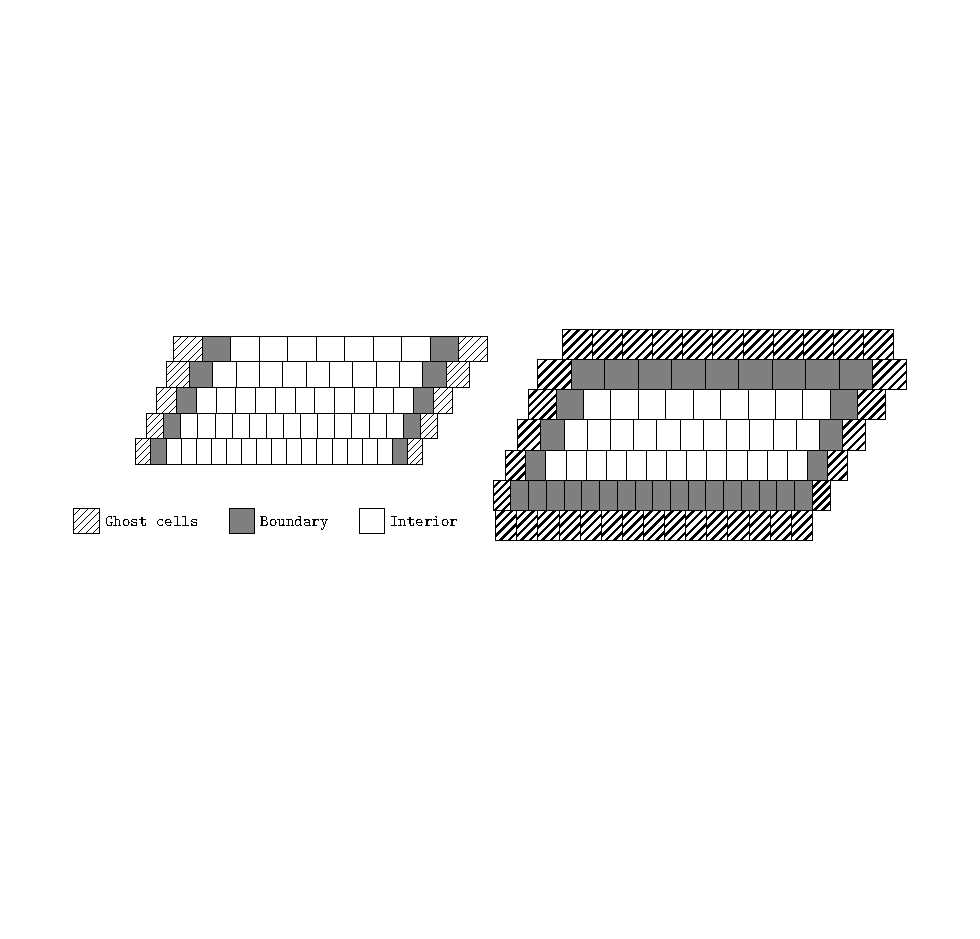
\includegraphics[width=8.5cm]{gmd-2014-119-f16.pdf}
  \caption{Ghost, boundary and interior cells for zonal (left) and meridional
  (right) advection.\label{fig2:ghost_cells}}

\end{figure}%

%f17
\begin{figure*}[t]
  \centering
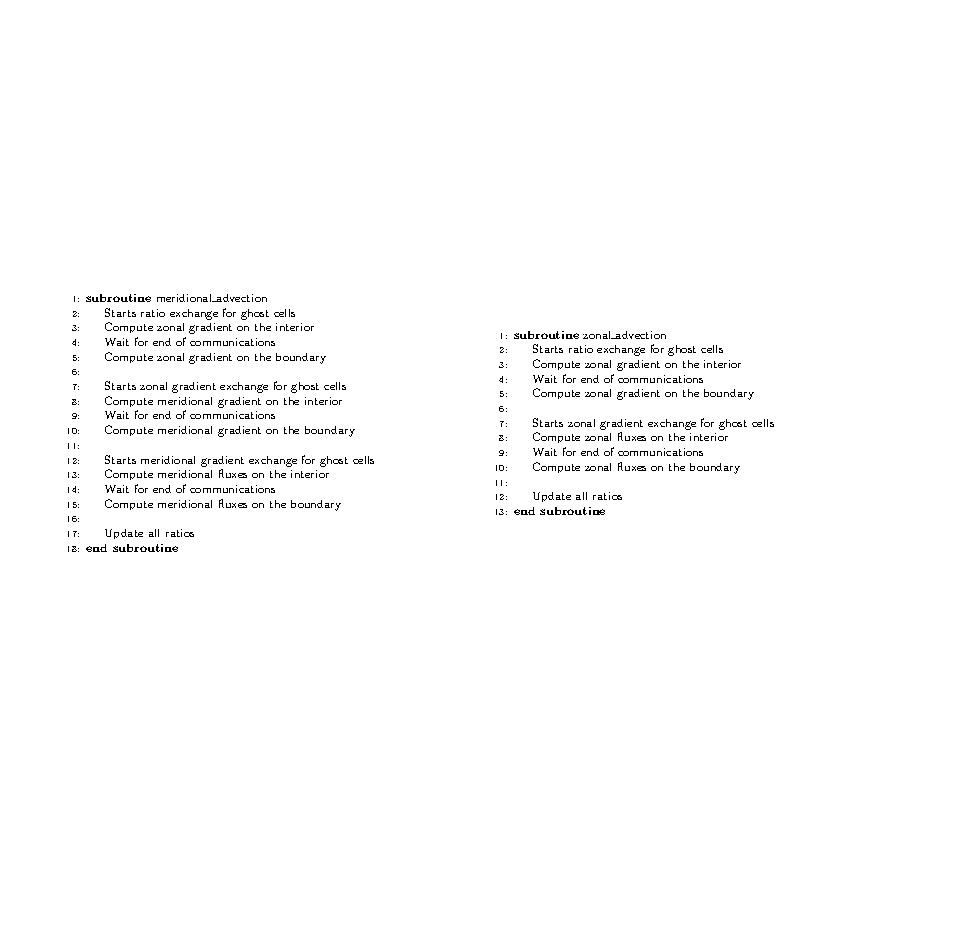
\includegraphics[width=14cm]{gmd-2014-119-f17.pdf}
    \label{algo:algo_merid}%
    \caption{Main steps of the algorithm for zonal (left) and meridional (right) advection.}
    \label{fig2:algos}
\end{figure*}%




   In order to improve the parallel performance of the code and hide the
   communication time as much as possible, non-blocking communications are used.
   This avoids waiting for the completion of communications and allows for computations to be optimized. In practice, we first post the communication
   requests, and then perform the calculation on the interior cells, which do not need data
   outside the current subdomain.  Then we finalize data reception and
   eventually compute the new quantities on the boundary cells using the values
   received in the ghost cells.  This approach is a~rather classical
   implementation to overlap computation and communication in large-scale
   simulations.  The specificity of Pangolin comes rather from the algebraic
   features of the decomposition, so the neighbors of a subdomain and the cells
   inside it are computed on the fly.  The model was also designed to have only
   one layer of ghost-cells as to decrease the communication volume.

   Each advection step can be decomposed into several tasks: gradient
   computing, fluxes computing and mass update. The first two tasks
   require some communication and the non-blocking approach is used
   for each one of them. It should be noted that meridional advection
   requires an extra communication as it needs a~zonal gradient to
   perform an interpolation (see Sect.~\ref{subsec:adapting}). The
   different tasks are shown in detail in the algorithms shown in
   Fig.~\ref{fig2:algos}. The combination of boundary and
   interior cells for all these tasks is shown in Fig.~\ref{fig2:ghost_cells}.

   The boundary zone is much larger for meridional advection as data
   need to be exchanged with the zone's four neighbors. More precisely,
   computation of the zonal gradient requires communication with the
   east and west neighbors of the subdomain. Furthermore, computing
   the meridional gradient and fluxes requires access to the north and
   south neighbors. Due to the semi-structured layout of the grid,
   this results in the ``stair-like'' structure for boundary cells in
   the meridional advection.

   Most of the computation is performed during meridional
   advection. First, due to the extra step of computing the zonal
   gradient, meridional advection requires three message exchanges (vs.
   two for zonal advection). Also, the number of boundary cells is
   larger, thus increasing the communication volume. Finally,
   computation in a~cell is more expensive as the number of neighbors
   is four on average (vs. two in the zonal case).

   \subsection{Performances}
   \label{subsec:performances}


%t3
\begin{table}[t]
\caption{Configuration for one of the 158 Sandy Bridge nodes.}
%\scalebox{.85}[.85]
  \centering
\begin{tabular}{p{7cm}} 
  \toprule
-- 2 Intel Sandy Bridge 8-core CPUs\par
\quad (peak performance of 330\,GFLOPS\,s$^{-1}$)\\
-- 32\,GB of memory\\
-- 31\,KB L1 cache, 256\,KB L2 cache for each core\\
-- 20\,MB L3 cache, shared by the 8 cores of each CPU\\
\bottomrule
\end{tabular}
%\belowtable
\label{tab:cluster}
\end{table}
   In this section, we investigate the parallel scalability of our
   implementation of the numerical scheme. Tests were done on the Bull
   cluster at CERFACS, whose features are shown in
   Table~\ref{tab:cluster}.  We consider a~strong speedup study where
   the size of the global grid is fixed and the number of computing
   cores is increased.  Ideally, the parallel elapsed time should be
   reduced proportionally to the number of cores selected for the
   parallel simulation.  For our experimental study, we consider the
   elapsed time on three cores as the reference time so that the
   speedup is defined by
\begin{align*}
 S(p) = \frac{T(3)}{T(p)},
   \end{align*}
   where $T(p)$ is the parallel elapsed time observed when performing
   the calculation on $p$ cores.

   In strong speedup studies, the number of cells per subdomain decreases when
   the number of subdomains increases. Even though we attempt to overlap the
   communication and the calculation, communication volume tends to grow when
   the number of subdomains increases. A~direct consequence is that the observed
   speedups gradually depart from the ideal speedup when the number of cores
   increases, as can be observed in Fig.~\ref{fig2:speedup} (left-hand side).
   On the right plot, we report experiments for the 2-D advection scheme using
   various grid sizes ranging from $1.13{\degre} \times 0.75{\degre}$ to
   $0.28{\degre} \times 0.19{\degre}$ when the number of cores varies from 3
   to 128. As expected, the larger the grid, the better the parallel
   performance, since we can better overlap calculation and computation. The speedup curves
   exhibit steps, with significant gaps when an optimal number of cores (6, 24,
   54, 96) is used. In between, using more cores does not translate into an
   improvement in performance as the workload of the largest subdomain is not
   reduced.

%f18
\begin{figure*}[t]
  \centering
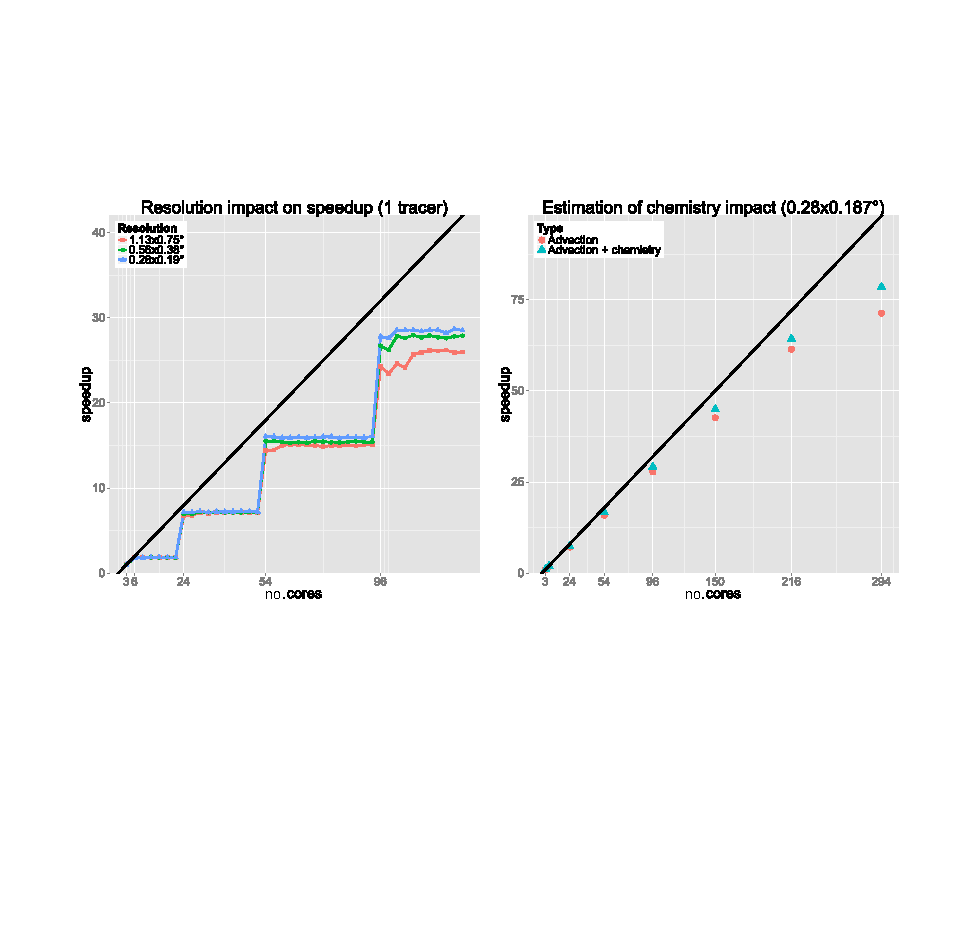
\includegraphics[width=14.5cm]{gmd-2014-119-f18.pdf}
  \caption{Speedup up to 126 cores (left) and 294 cores (right).  The left plot
    shows the impact of grid resolution for smaller configurations. The right
    plot shows both the advection performances and an estimation of the
    chemistry impact on scalability. Resolutions used are
    $1.125{\degre}\times0.75\degre$, $0.56{\degre}\times0.376\degre$ and
    $0.28{\degre}\times0.188\degre$. Both figures use non-divergent winds from
    Sect.~\ref{sec2:tests} over a~full period with a~CFL of 0.96.
  }
  \label{fig2:speedup}%
\end{figure*}%

%f19
\begin{figure}[t]
  \centering
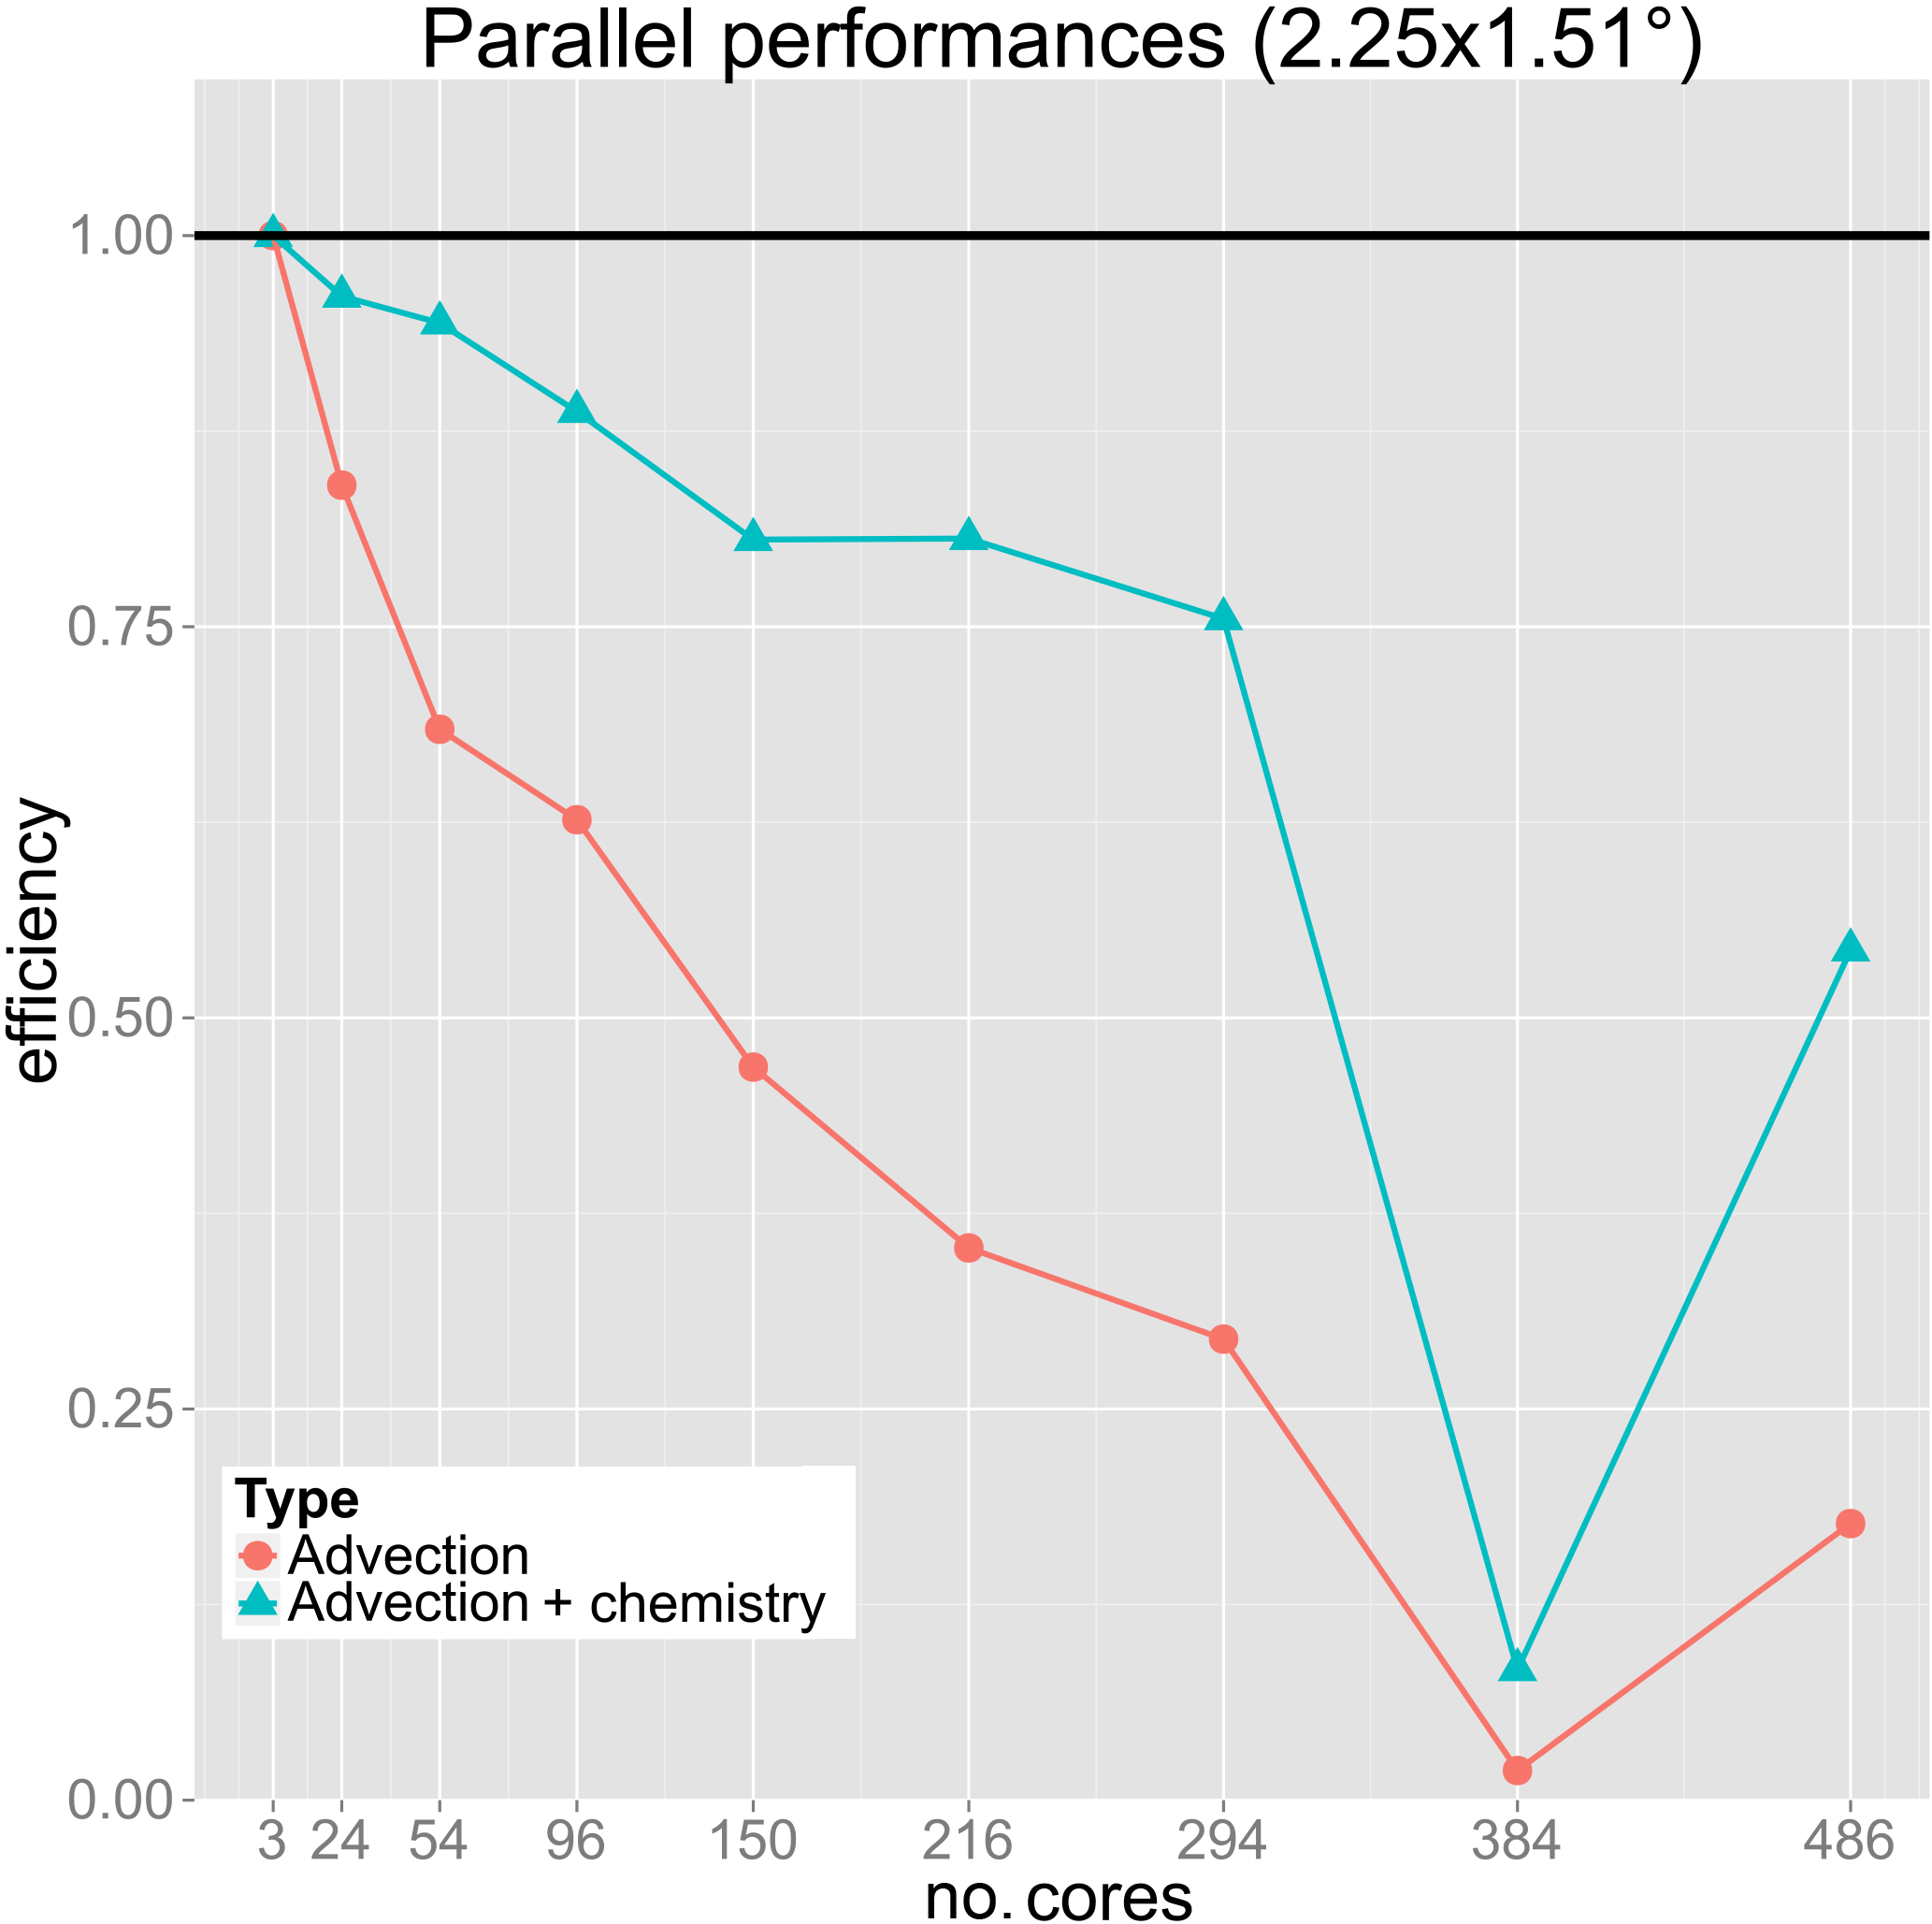
\includegraphics[width=8.5cm]{gmd-2014-119-f19.png}
  \caption{Efficiency up to 486 cores. A resolution of
    $2.25\times1.51\degre$ was used to examine the limit of the parallelization
    performances for 2-D advection. For this test, the Airain cluster was used,
    which has 9504 nodes where each node has an Intel Xeon processor (16 cores,
2.7\,GHz and 4\,GB of shared memory).}
  \label{fig2:efficiency}%
\end{figure}

   The final version of Pangolin will be combined with chemistry modeling. As
   the chemistry computation is fully local, we can estimate the performances of
   the chemistry-advection model. Figure~\ref{fig2:speedup} (right-hand side)
   shows the estimated speedups of the complete chemistry advection simulation
   on the finest grid (i.e., $0.28{\degre} \times 0.19{\degre}$). We assumed
   the chemistry cost was constant across all cells and the chemical time step
   was similar to the advection time step.  These assumptions are not valid in
   practice and only give an upper bound on the speedup. Nevertheless they give
   some insight into the final performances.  The chemical time step was obtained
   from a~new solver developed by D.~Cariolle (personal communication, 2014)
   called ASIS with 90 species. As a~reference, we use its implementation by P.
   Moinat, using the GMRES method (personal communication, 2014). As a~result,
   adding the chemistry greatly increases the computational load in a~subdomain
   and thus improves the scalability. On the other hand, communication volumes
   only increase linearly as a~function of the number of tracers, as expected.

   Comparing performances between parallel models is not an easy task. A
   meaningful comparison would require all of the models to be compiled and run on the
   same cluster as hardware and software performances are paramount in such
   studies. Such tests are not within the scope of the current paper. However, we
   examine the limits of our parallelization strategy, an additional strong scaling
   test was run with a rather coarse resolution ($2.25\times1.75\degre$): the
   number of cores was increased until the subdomains became extremely small. At that
   point, the computational load inside the subdomains is not enough to cover
   the communication costs. These results are shown in
   Fig.~\ref{fig2:efficiency},
   where the efficiency is plotted against the number of cores. Here, the
   efficiency is defined as
   \begin{align*}
     E(p) = \frac{T(3)}{p T(p)},
   \end{align*}
   so ideal performances should be close to $1$. We can consider the parallel
   performances ``break down'' at 294 cores. The size of the subdomains is then
   $5\times5$, a non-realistic configuration where the subdomains are so small
   that the communication cost can no longer be hidden. From this test, we have
   estimated the size of subdomains needed for an efficiency of $0.75$ was
   $18\times18$.  In practice, this allowed us to estimate the number of cores
   needed for the same efficiency at different resolutions. Results are shown in
   Table~\ref{table:nb_cores}.


%t4
   \begin{table}[t]
     \begin{minipage}[b]{0.45\linewidth}
       \caption{Estimation of the number of cores needed for an efficiency of $0.75$ for
       2-D advection at several resolutions (lat\,$\times$\,long).}
       \centering
       \begin{tabular}{cc}
         \toprule
         Resolution & No. cores \\
         \midrule
         $1.5\times1.0$ & 150  \\
         $0.75\times0.5$ & 486 \\
         $0.15\times0.1$ & 6144 \\
         \bottomrule
       \end{tabular}
       \label{table:nb_cores}
     \end{minipage}
     \hfill
     \begin{minipage}[b]{0.5\linewidth}
       \caption{Some Pangolin configurations, with  the number of latitudes on a
         hemisphere $n_{\text{lat}}$, total number of cells $n_{\text{pangolin}}$ and
       resolution at the Equator in degrees.}
       \centering
       \begin{tabular}{rrc}
         \toprule
         $n_{\text{lat}}$ & $n_{\text{pangolin}}$ & $\Delta\phi \times \Delta\lambda$\\
         \midrule
         20   & 2400   & $4.5  \times 3.08$  \\
         90   & 48\,600  & $1.0  \times 0.67$  \\
         320  & 614\,400 & $0.28 \times 0.188$\\
         \bottomrule
       \end{tabular}
       \label{table:pango_res}
     \end{minipage}
   \end{table}

  \section{Conclusions}
   \label{sec2:ccl}

   In this paper, we have presented a~parallel scalable algorithm for
   2-D-advection on the sphere. We focused on enabling the model to be as
   parallel as possible. Pangolin uses a~reduced latitude--longitude grid, which
   overcomes the pole issue, and a~finite-volume formulation that ensures local
   conservation of the tracer mass.  Grid features were carefully exploited to
   minimize memory requirements on the one hand, and provide maximal efficiency on
   parallel architectures on the other. The accuracy of the scheme was also
   chosen as to minimize the impact on message passing. It was found that the
   approximations made for computing the meridional gradients near the poles
   limits the accuracy of the model. Therefore, to reach the accuracy of other
   second-order models, resolution must be increased. This can be easily
   achieved without large computation penalty due to the good scalability of
   Pangolin.

   We expect further improvement in terms of parallelism when chemistry is
   added. An ongoing work addresses real-case atmospheric situations using a
   linear scheme (\cite{Cariolle2007}), which is used to model the evolution of
   stratospheric ozone on an isentropic surface. In future versions, vertical
   advection will be added, requiring a more advanced correction of the winds
   for mass preservation. A complex chemistry will also be added using the ASIS
   solver and the RACMOBUS scheme (\cite{Dufour2005}). This chemistry will most
   likely perturb the load balancing. One mitigation strategy would be to use
   multi-threading in the subdomains. To conclude, Pangolin is a practical
   model that is aimed at taking advantage of present and future parallel
   architectures for large-scale atmospheric transport.


   \section*{Code availability}

   The code is copyright of the CERFACS laboratory. The
   documentation is available as a~user manual and as code
   documentation at
   \url{http://cerfacs.fr/~praga/pangolin/index.html}.  To request
   access to either the source code or documentation, please email A.~Praga (alexis.praga@gmail.com) or D.~Cariolle
    (cariolle@cerfacs.fr).  The data and scripts for the plots of this
   paper are also available as a~supplement.

   \section*{Acknowledgements}
  Financial support from the DGAC (Direction G\'en\'erale de l'Aviation Civile)
  through the project IMPACT is gratefully acknowledged. A.~Praga was supported
  by a~PhD grant from M\'et\'eo-France.\newline\newline Edited by: A.~Colette
